\section{Risultati ottenuti}
In questa sezione vengono riportati i risultati ottenuto eseguendo le diverso simulazioni presentate precedentemente. In particolare, per ogni casistica di studio (Random, Betweenness, Eigenvector) vengono riportate statistiche relative alla diffusione dell'informazione, fornendo una panoramica sulla distribuzione di utenti non esposti, esposti e infetti, e delle rispettive tipologie di contagio.
    \subsection{Random}
    Vengono di seguito riportati i risultati relativi alle simulazioni basate su scelta randomica del posizionamento dei Bot.
        \subsubsection{Grafo da 500 follower}

            \begin{figure}[H]
                \centering
                \begin{minipage}[c]{0.55\textwidth}
                    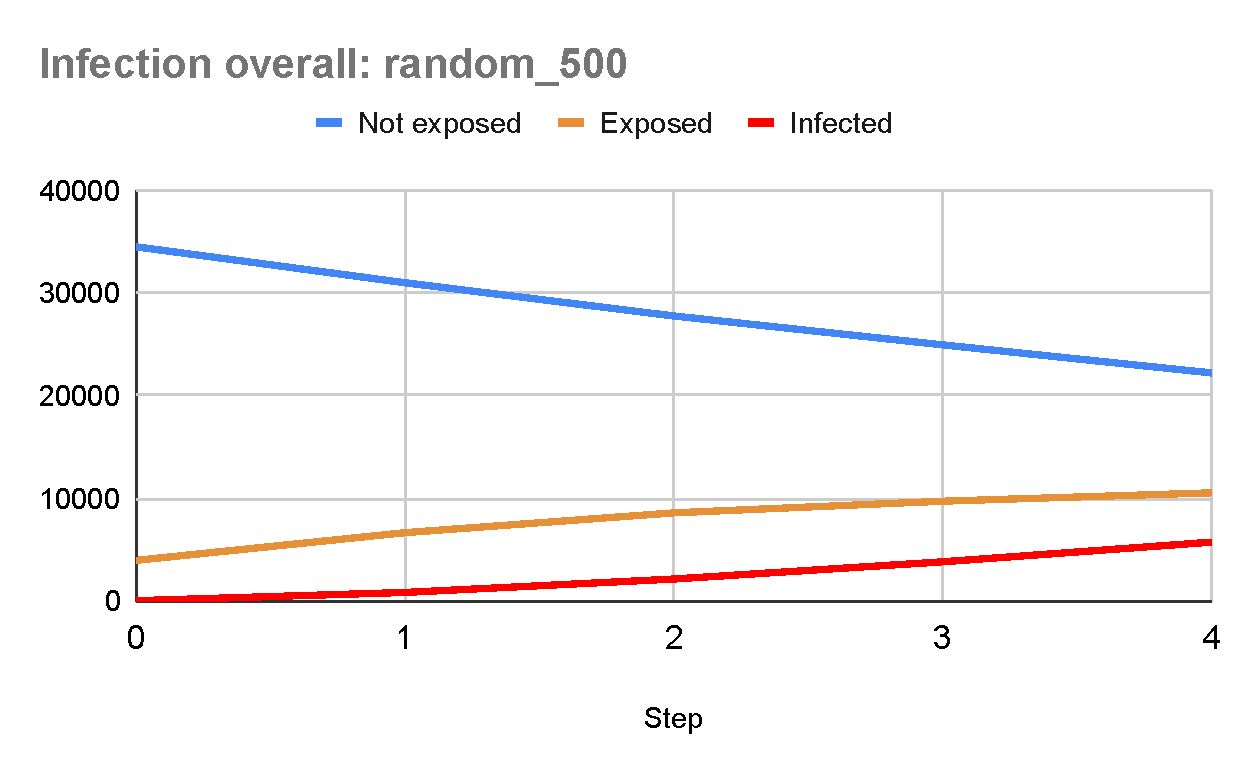
\includegraphics[width=\textwidth]{resources/charts/Infection overall_ random_500.pdf}
                \end{minipage}
                \hfill
                \begin{minipage}[c]{0.44\textwidth}
                    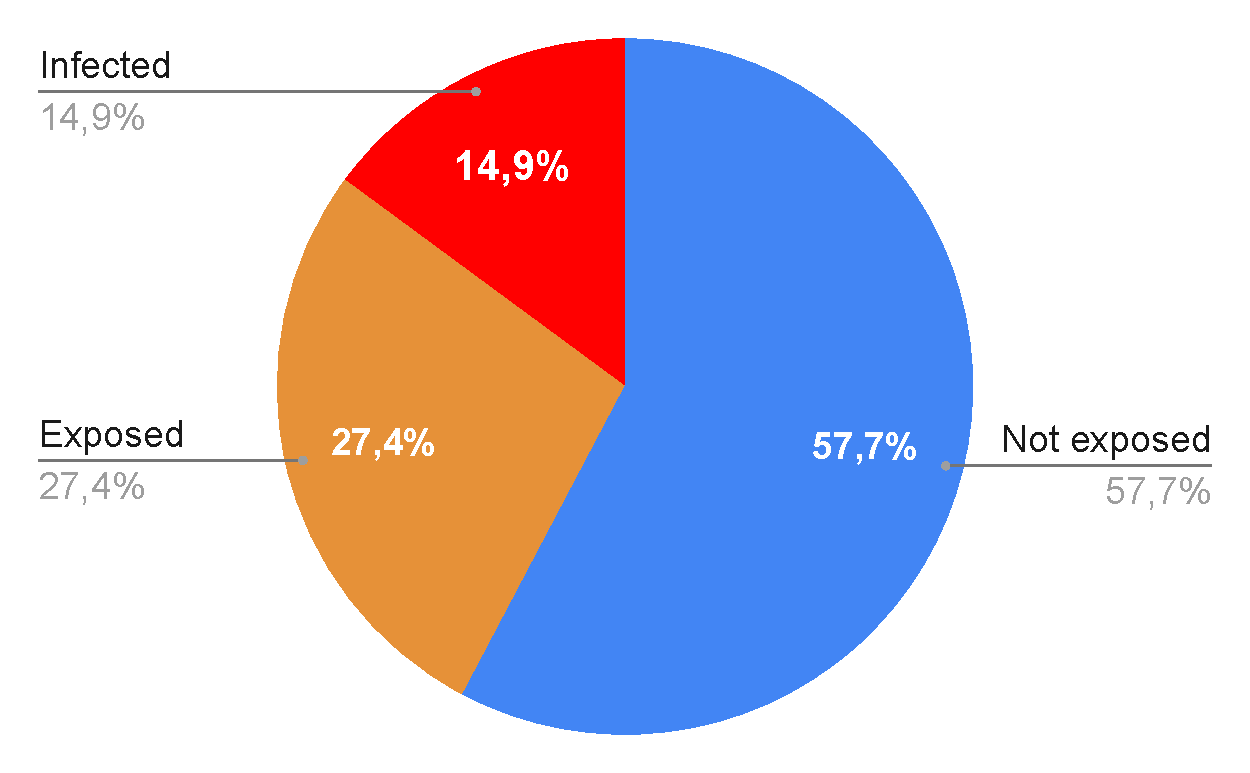
\includegraphics[width=\textwidth]{resources/charts/pie_random_500.pdf}
                \end{minipage}
                \caption{Andamento della diffusione dell'informazione. Simulazione random\_500.}
            \end{figure}
            
            \begin{table}[H]
                \centering
                \begin{tabular}{l|c|c|c|c|c}
                            & Step 0 & Step 1 & Step 2 & Step 3 & Step 4 \\ \hline
                \textbf{Not exposed} & 34487  & 30989  & 27757  & 24945  & 22214  \\ \hline
                \textbf{Exposed}     & 3964   & 6659   & 8586   & 9721   & 10538  \\ \hline
                \textbf{Infected}    & 34     & 837    & 2142   & 3819   & 5733   \\
                \end{tabular}
                \caption{Numero di nodi non esposti/esposti/infetti in relazione agli step della simulazione random\_500.}
            \end{table}
            
        \begin{figure}[H]
            \centering
            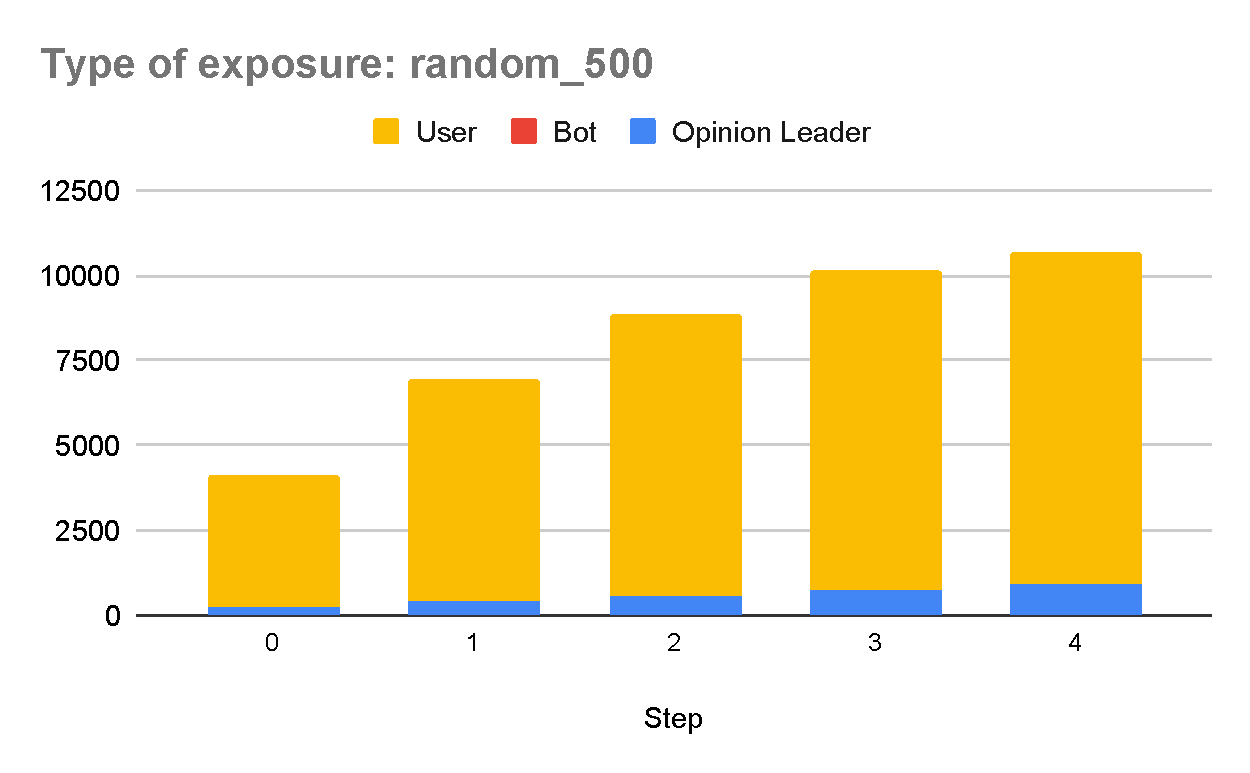
\includegraphics[width=.7\textwidth]{resources/charts/Type of exposure_ random_500.pdf}
            \caption{Tipologia di esposizione all'informazione durante ogni fase della simulazione random\_500.}
        \end{figure}
        
        \begin{table}[H]
            \centering
            \begin{tabular}{l|c|c|c|c|c}
                           & Step 0 & Step 1 & Step 2 & Step 3 & Step 4 \\ \hline
            \textbf{Opinion Leader} & 278    & 456    & 600    & 791    & 957    \\ \hline
            \textbf{Bot}            & 1      & 1      & 1      & 0      & 5      \\ \hline
            \textbf{User}           & 3828   & 6512   & 8235   & 9311   & 9744   \\
            \end{tabular}
            \caption{Numero di nodi responsabili dell'esposizione in base alla tipologia e allo step di esecuzione della simulazione random\_500.}
        \end{table}

    \subsubsection{Grafo da 1000 follower}
        \begin{figure}[H]
            \centering
            \begin{minipage}[c]{0.55\textwidth}
                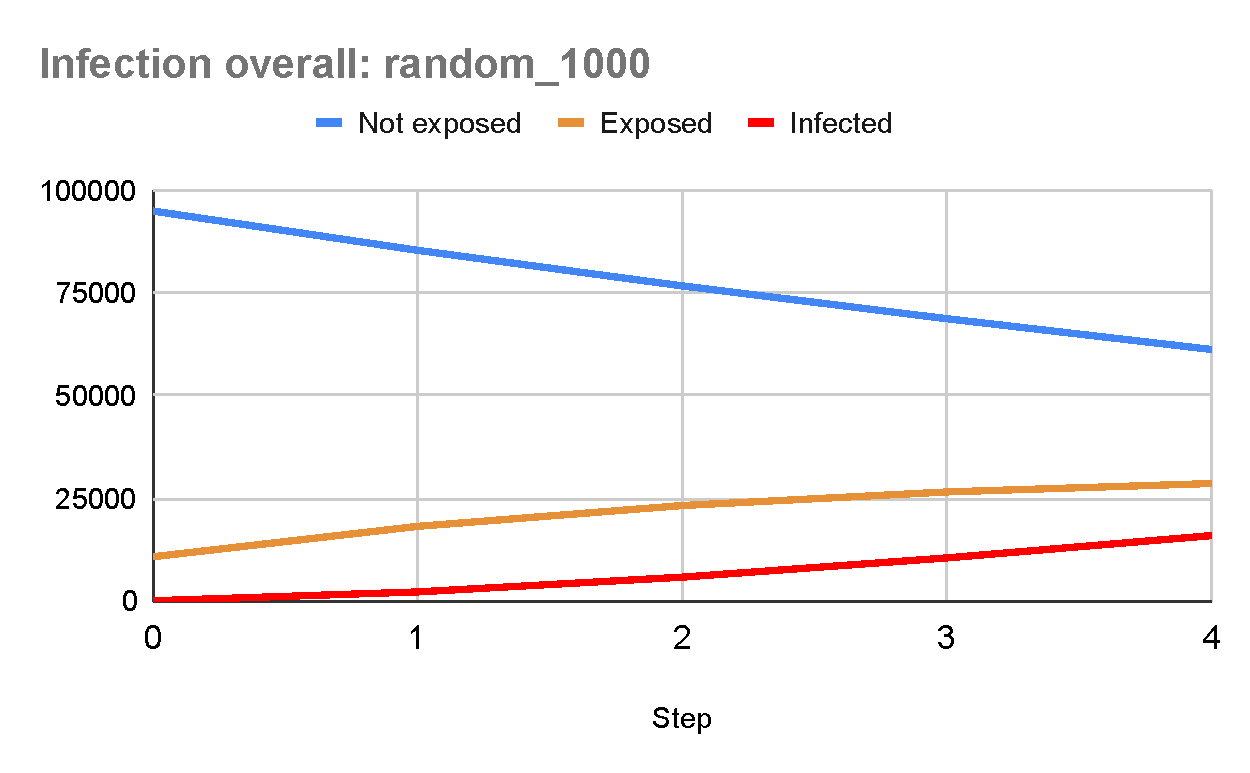
\includegraphics[width=\textwidth]{resources/charts/Infection overall_ random_1000.pdf}
            \end{minipage}
            \hfill
            \begin{minipage}[c]{0.44\textwidth}
                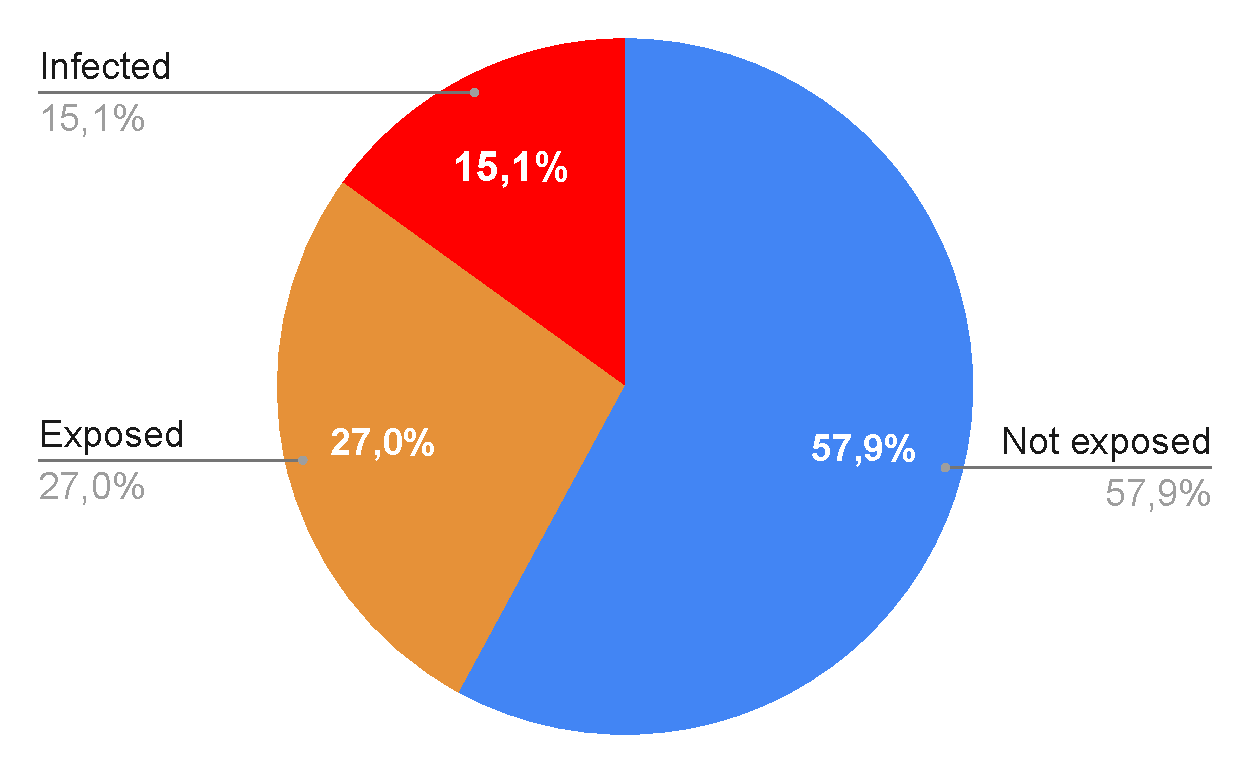
\includegraphics[width=\textwidth]{resources/charts/pie_random_1000.pdf}
            \end{minipage}
            \caption{Andamento della diffusione dell'informazione. Simulazione random\_1000.}
        \end{figure}
        
        \begin{table}[H]
            \centering
            \begin{tabular}{l|c|c|c|c|c}
                        & Step 0 & Step 1 & Step 2 & Step 3 & Step 4 \\ \hline
            \textbf{Not exposed} & 94933  & 85375  & 76715  & 68726  & 61240  \\ \hline
            \textbf{Exposed}     & 10783  & 18178  & 23246  & 26555  & 28607  \\ \hline
            \textbf{Infected}    & 58     & 2221   & 5813   & 10493  & 15927  \\
            \end{tabular}
            
            \caption{Numero di nodi non esposti/esposti/infetti in relazione agli step della simulazione random\_1000.}
        \end{table}

        \begin{figure}[H]
            \centering
            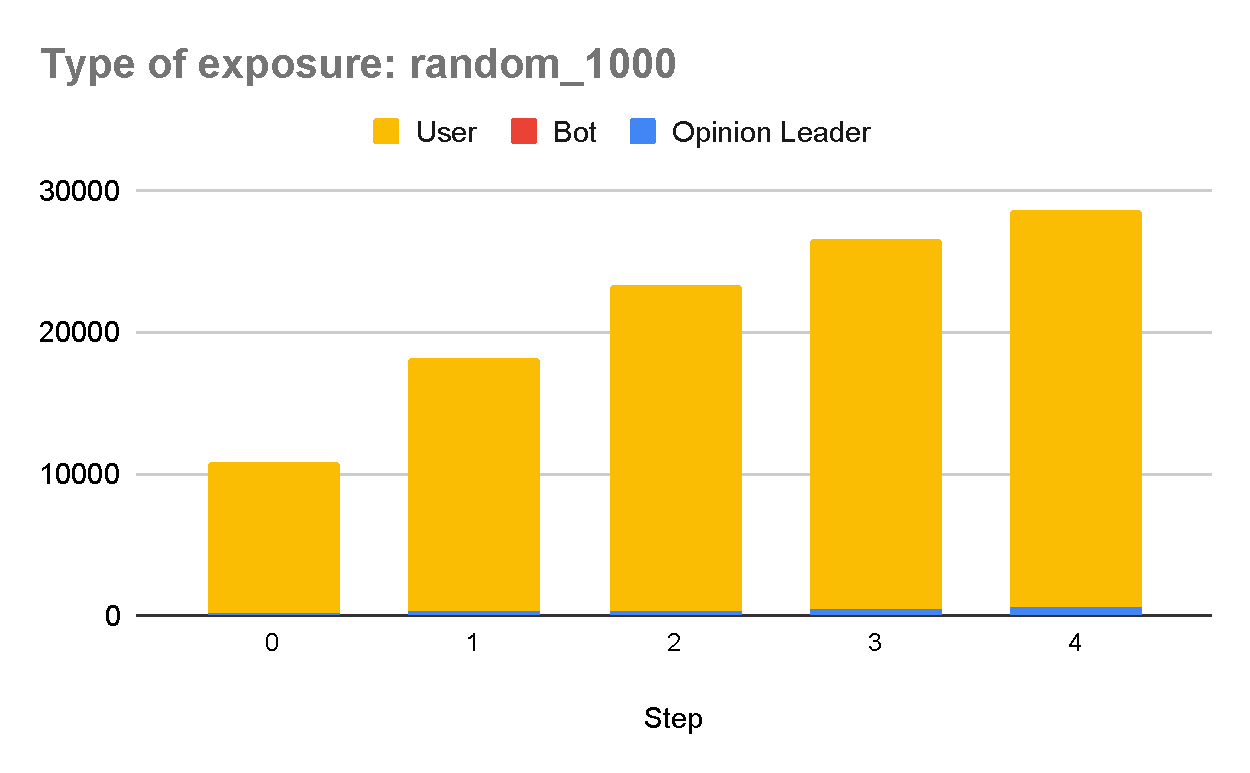
\includegraphics[width=.7\textwidth]{resources/charts/Type of exposure_ random_1000.pdf}
            \caption{Tipologia di esposizione all'informazione durante ogni fase della simulazione random\_1000.}
        \end{figure}
        
        \begin{table}[H]
            \centering
            \begin{tabular}{l|c|c|c|c|c}
                           & Step 0 & Step 1 & Step 2 & Step 3 & Step 4 \\ \hline
            \textbf{Opinion Leader} & 259    & 352    & 355    & 547    & 631    \\ \hline
            \textbf{Bot}            & 0      & 0      & 0      & 0      & 0      \\ \hline
            \textbf{User}           & 10524  & 17826  & 22891  & 26008  & 27976  \\
            \end{tabular}
            \caption{Numero di nodi responsabili dell'esposizione in base alla tipologia e allo step di esecuzione della simulazione random\_1000.}
        \end{table}

    \subsubsection{Grafo da 1500 follower}
        \begin{figure}[H]
            \centering
            \begin{minipage}[c]{0.55\textwidth}
                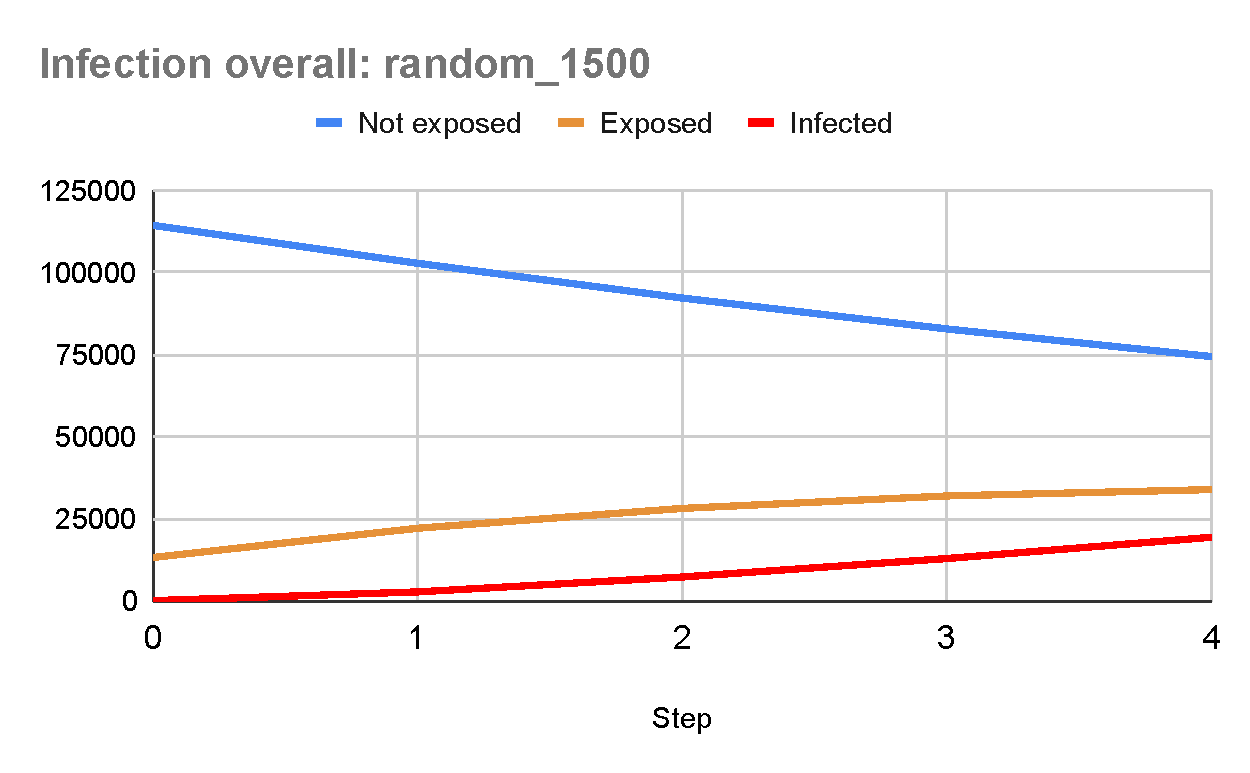
\includegraphics[width=\textwidth]{resources/charts/Infection overall_ random_1500.pdf}
            \end{minipage}
            \hfill
            \begin{minipage}[c]{0.44\textwidth}
                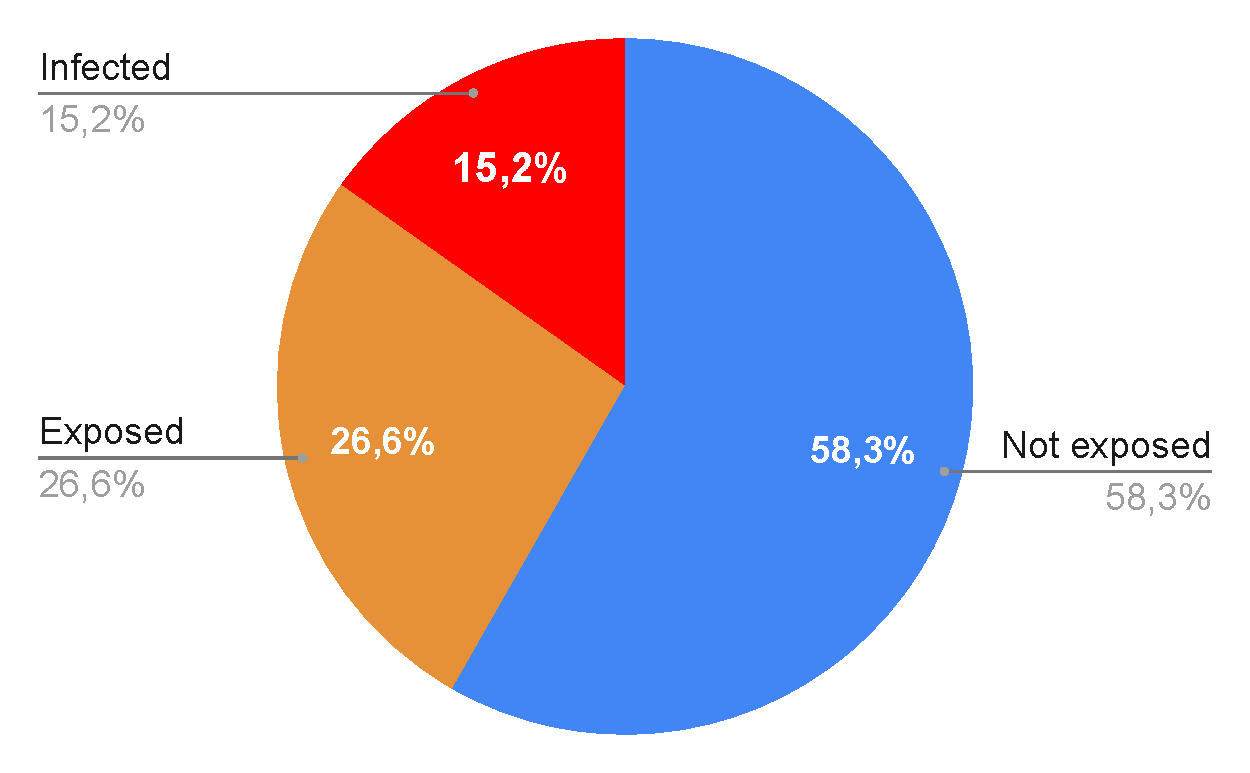
\includegraphics[width=\textwidth]{resources/charts/pie_random_1500.pdf}
            \end{minipage}
            \caption{Andamento della diffusione dell'informazione. Simulazione random\_1500.}
        \end{figure}
            
        \begin{table}[H]
            \centering
            \begin{tabular}{l|c|c|c|c|c}
                        & Step 0 & Step 1 & Step 2 & Step 3 & Step 4 \\ \hline
            \textbf{Not exposed} & 114324 & 102770 & 92206  & 82798  & 74386  \\ \hline
            \textbf{Exposed}     & 13261  & 22151  & 28184  & 31974  & 33914  \\ \hline
            \textbf{Infected}    & 115    & 2779   & 7310   & 12928  & 19400  \\
            \end{tabular}
            \caption{Numero di nodi non esposti/esposti/infetti in relazione agli step della simulazione random\_1500.}
        \end{table}
        
        \begin{figure}[H]
            \centering
            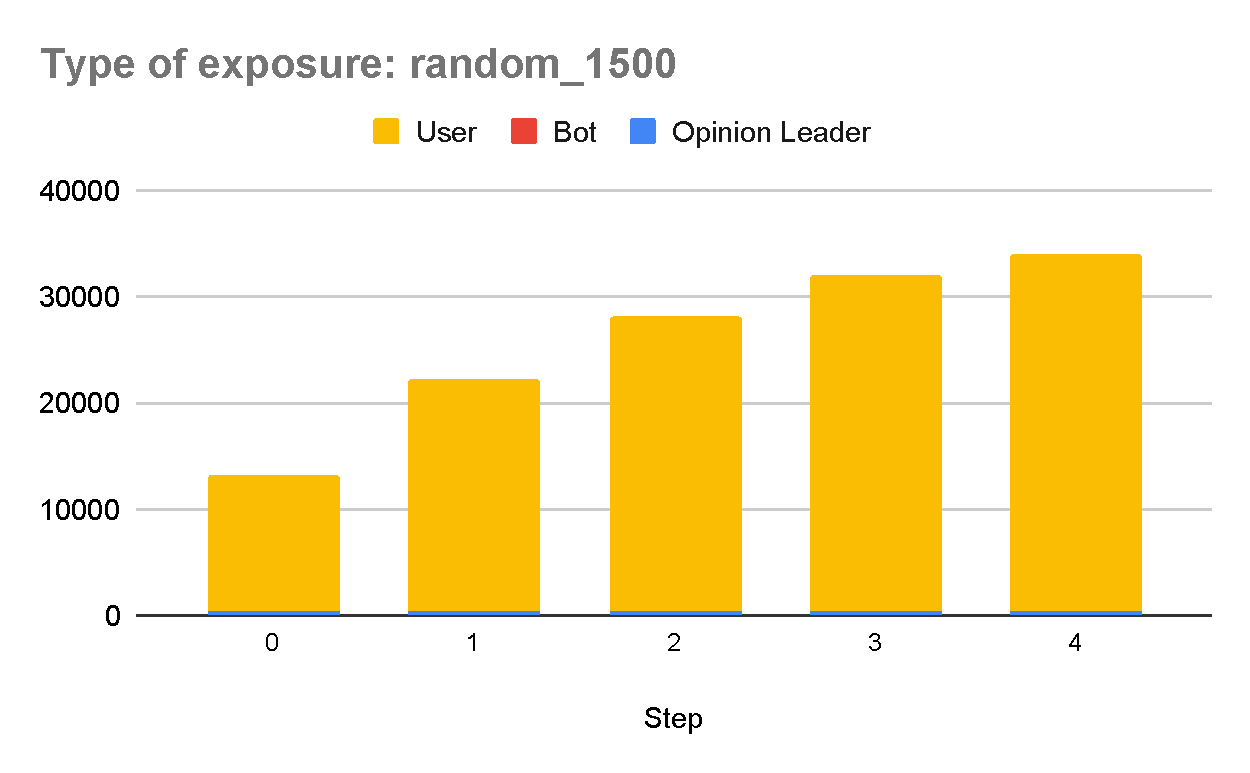
\includegraphics[width=.7\textwidth]{resources/charts/Type of exposure_ random_1500.pdf}
            \caption{Tipologia di esposizione all'informazione durante ogni fase della simulazione random\_1500.}
        \end{figure}
        
        \begin{table}[H]
            \centering
            \begin{tabular}{l|c|c|c|c|c}
                           & Step 0 & Step 1 & Step 2 & Step 3 & Step 4 \\ \hline
            \textbf{Opinion Leader} & 418    & 516    & 502    & 510    & 471    \\ \hline
            \textbf{Bot}            & 0      & 0      & 0      & 0      & 0      \\ \hline
            \textbf{User}           & 12843  & 21635  & 27682  & 31464  & 33443  \\
            \end{tabular}
            \caption{Numero di nodi responsabili dell'esposizione in base alla tipologia e allo step di esecuzione della simulazione random\_1500.}
        \end{table}

    \subsubsection{Grafo da 2000 follower}

        \begin{figure}[H]
            \centering
            \begin{minipage}[c]{0.55\textwidth}
                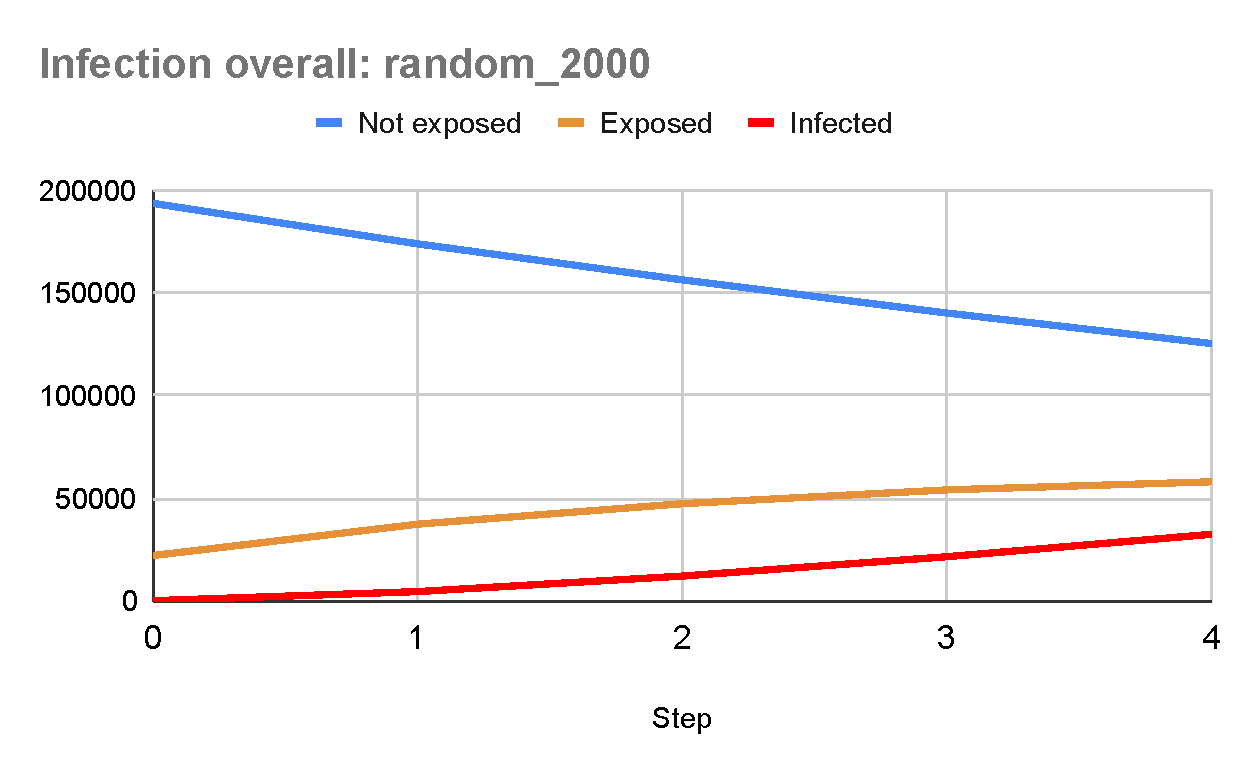
\includegraphics[width=\textwidth]{resources/charts/Infection overall_ random_2000.pdf}
            \end{minipage}
            \hfill
            \begin{minipage}[c]{0.44\textwidth}
                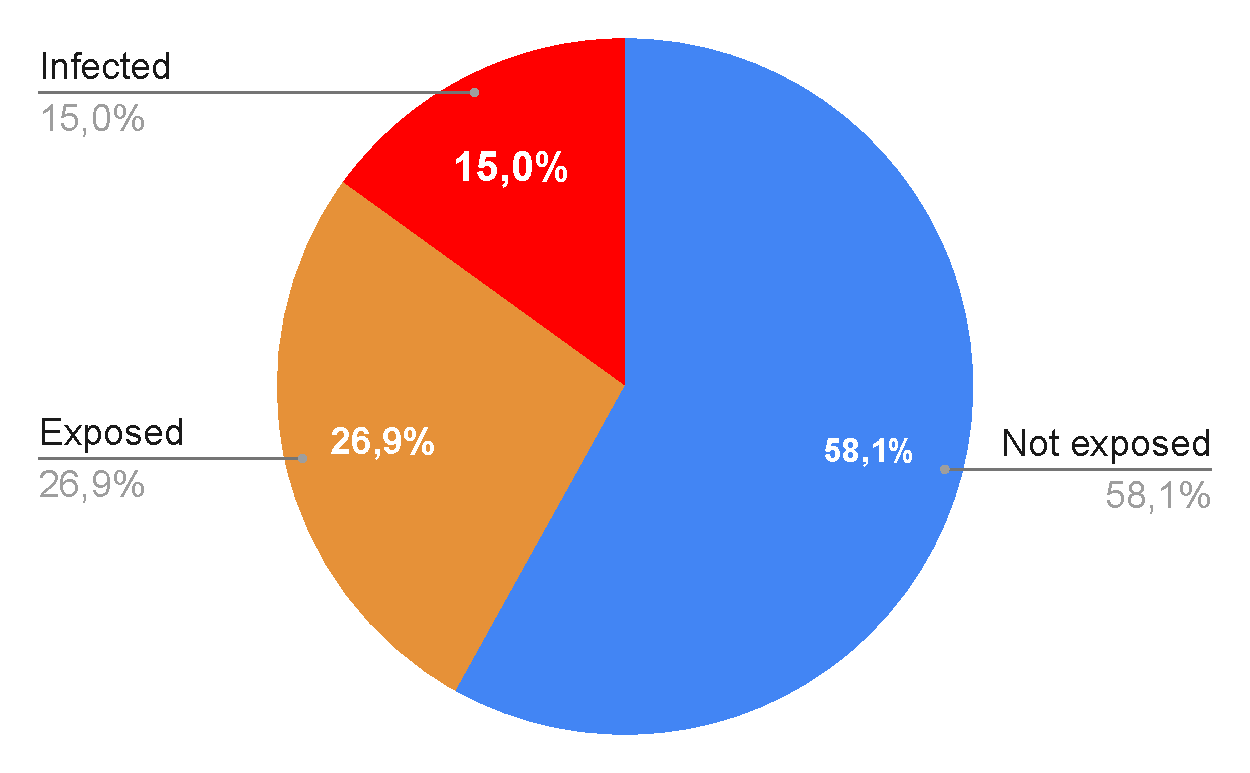
\includegraphics[width=\textwidth]{resources/charts/pie_random_2000.pdf}
            \end{minipage}
            \caption{Andamento della diffusione dell'informazione. Simulazione random\_2000.}
        \end{figure}
        
        \begin{table}[H]
            \centering
            \begin{tabular}{l|c|c|c|c|c}
                        & Step 0 & Step 1 & Step 2 & Step 3 & Step 4 \\ \hline
            \textbf{Not exposed} & 193592 & 173891 & 156381 & 140232 & 125366 \\ \hline
            \textbf{Exposed}     & 22155  & 37424  & 47383  & 54109  & 58054  \\ \hline
            \textbf{Infected}    & 163    & 4595   & 12146  & 21569  & 32490  \\
            \end{tabular}
            \caption{Numero di nodi non esposti/esposti/infetti in relazione agli step della simulazione random\_2000.}
        \end{table}
        
        \begin{figure}[H]
            \centering
            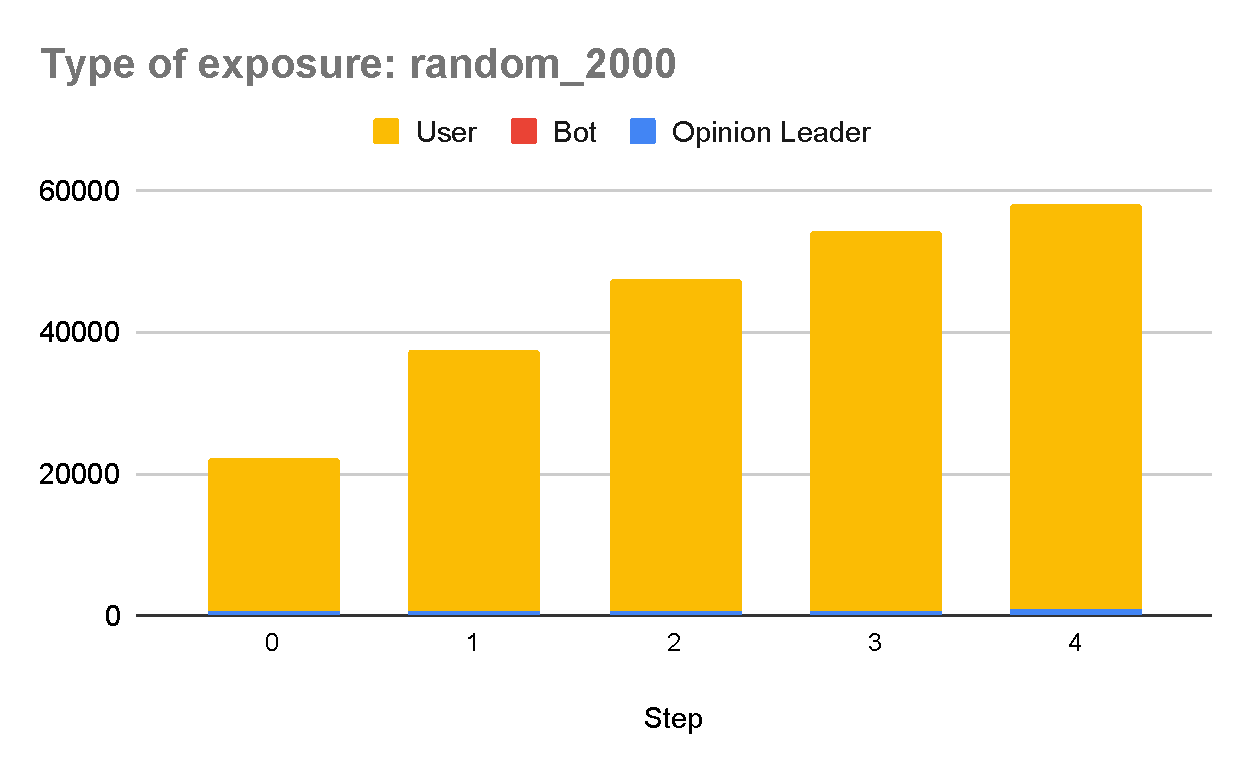
\includegraphics[width=.7\textwidth]{resources/charts/Type of exposure_ random_2000.pdf}
            \caption{Tipologia di esposizione all'informazione durante ogni fase della simulazione random\_2000.}
        \end{figure}
        
        \begin{table}[H]
            \centering
            \begin{tabular}{l|c|c|c|c|c}
                           & Step 0 & Step 1 & Step 2 & Step 3 & Step 4 \\ \hline
           \textbf{Opinion Leader} & 600    & 726    & 731    & 707    & 964    \\ \hline
            \textbf{Bot}            & 0      & 0      & 0      & 0      & 0      \\ \hline
            \textbf{User}           & 21555  & 36698  & 46652  & 53402  & 57090  \\
            \end{tabular}
            \caption{Numero di nodi responsabili dell'esposizione in base alla tipologia e allo step di esecuzione della simulazione random\_2000.}
        \end{table}
        
        \textbf{Considerazioni simulazioni Random} 
        
        La selezione randomica della posizione dei Bot non ha portato alcun contributo rispetto alla propagazione dell'informazione 
        poiché al termine della simulazione la percentuale di utenti non esposti risulta significativamente maggiore rispetto a quella degli utenti esposti o infetti.
        
        Notasi che questi stessi risultati sono stati ottenuti indipendentemente dalla variazione della topologia di grafo considerata.

    \subsection{Betweenness e In-Degree}
    Vengono di seguito riportati i risultati relativi alle simulazioni basate su scelta del posizionamento dei Bot rispetto alla misura della Betweenness. Si noti che in tutti i grafi considerati i nodi aventi maggiore Betweenness sono risultati essere coincidenti con quelli aventi maggiore In-Degree.
    
        \subsubsection{Grafo da 500 follower}
            
            \begin{figure}[H]
                \centering
                \begin{minipage}[c]{0.55\textwidth}
                    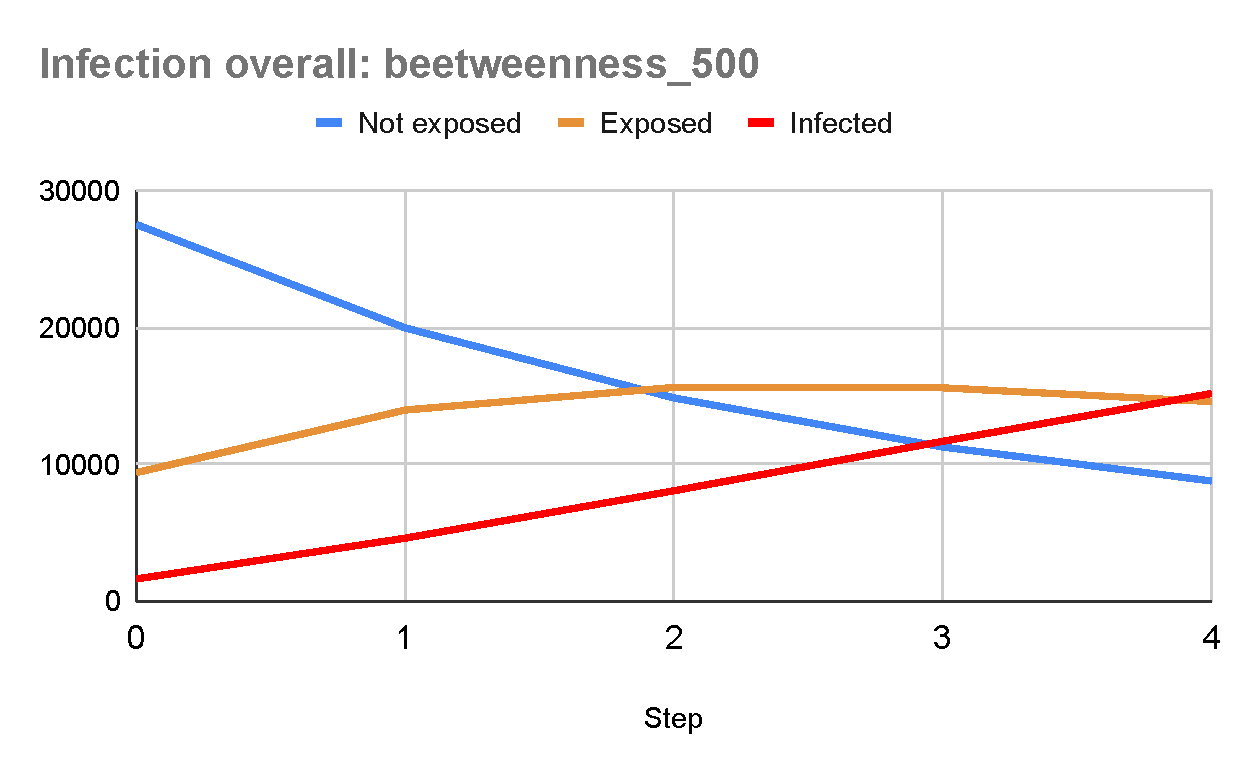
\includegraphics[width=\textwidth]{resources/charts/Infection overall_ beetweenness_500.pdf}
                \end{minipage}
                \hfill
                \begin{minipage}[c]{0.44\textwidth}
                    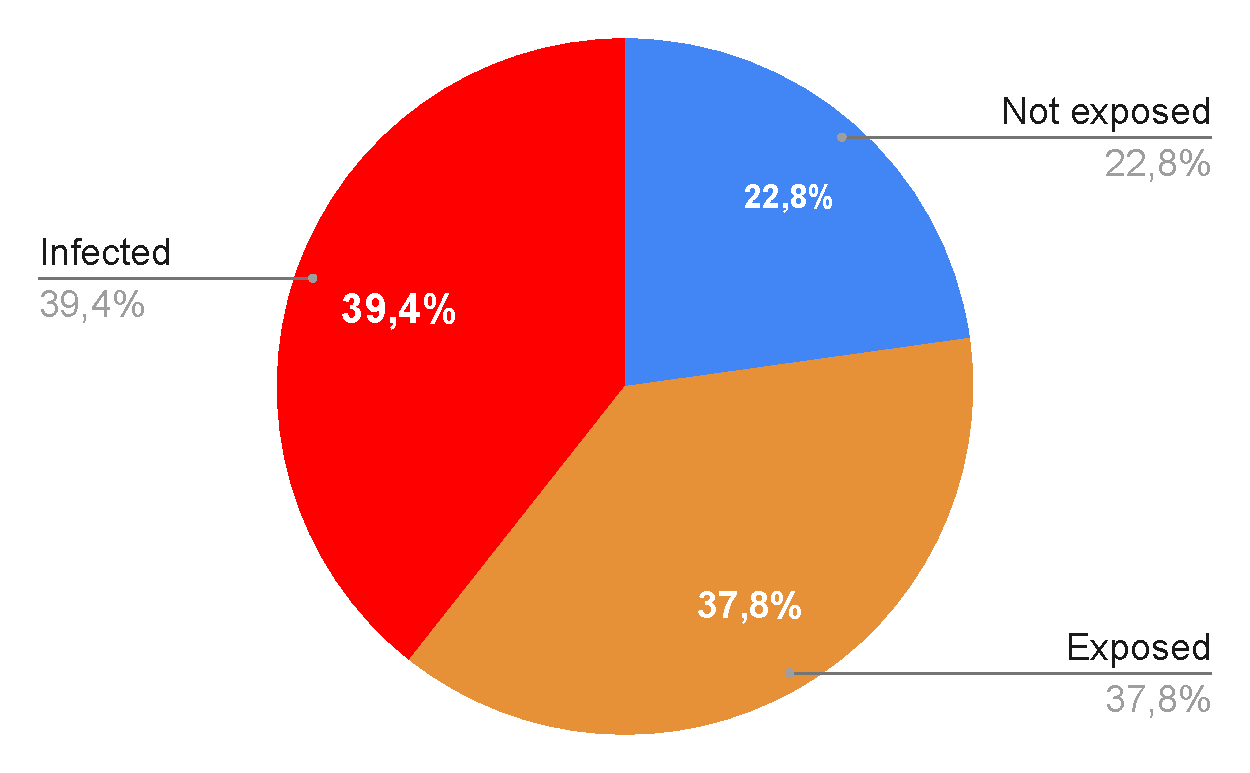
\includegraphics[width=\textwidth]{resources/charts/pie_btw_500.pdf}
                \end{minipage}
                \caption{Andamento della diffusione dell'informazione. Simulazione betweenness\_500.}
            \end{figure}
            
            
            \begin{table}[H]
                \centering
                \begin{tabular}{l|c|c|c|c|c}
                            & Step 0 & Step 1 & Step 2 & Step 3 & Step 4 \\ \hline
                \textbf{Not exposed} & 27493  & 19944  & 14833  & 11251  & 8769   \\ \hline
                \textbf{Exposed}     & 9380   & 13949  & 15600  & 15571  & 14564  \\ \hline
                \textbf{Infected}    & 1612   & 4592   & 8052   & 11663  & 15152  \\
                \end{tabular}
                \caption{Numero di nodi non esposti/esposti/infetti in relazione agli step della simulazione betweenness\_500.}
            \end{table}
            
            \begin{figure}[H]
                \centering
                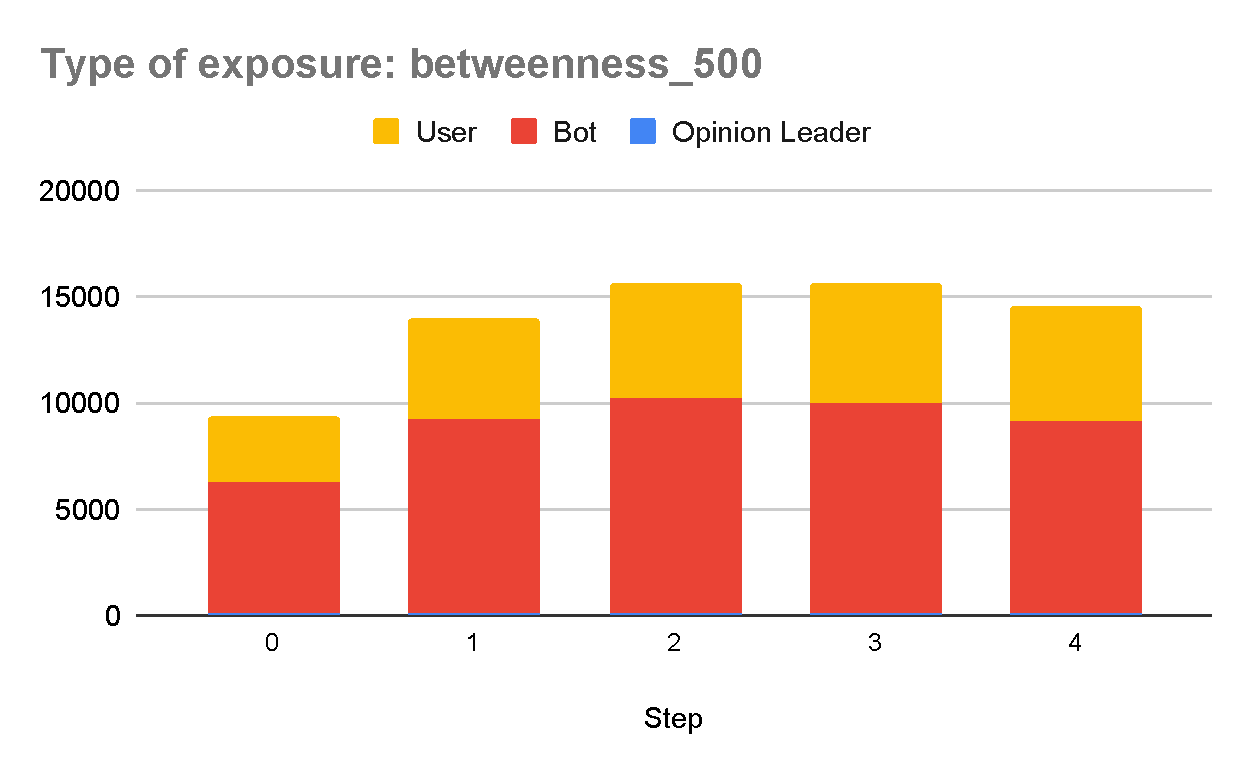
\includegraphics[width=.7\textwidth]{resources/charts/Type of exposure_ betweenness_500.pdf}
                \caption{Tipologia di esposizione all'informazione durante ogni fase della simulazione betweenness\_500.}
            \end{figure}
            
            \begin{table}[H]
                \centering
                \begin{tabular}{l|c|c|c|c|c}
                               & Step 0 & Step 1 & Step 2 & Step 3 & Step 4 \\ \hline
                \textbf{Opinion Leader} & 144    & 172    & 180    & 174    & 156    \\ \hline
                \textbf{Bot}            & 6152   & 9086   & 10035  & 9852   & 9015   \\ \hline
                \textbf{User}           & 3084   & 4691   & 5385   & 5545   & 5393   \\
                \end{tabular}
                \caption{Numero di nodi responsabili dell'esposizione in base alla tipologia e allo step di esecuzione della simulazione random\_500.}
            \end{table}

        \subsubsection{Grafo da 1000 follower}

            \begin{figure}[H]
                \centering
                \begin{minipage}[c]{0.55\textwidth}
                    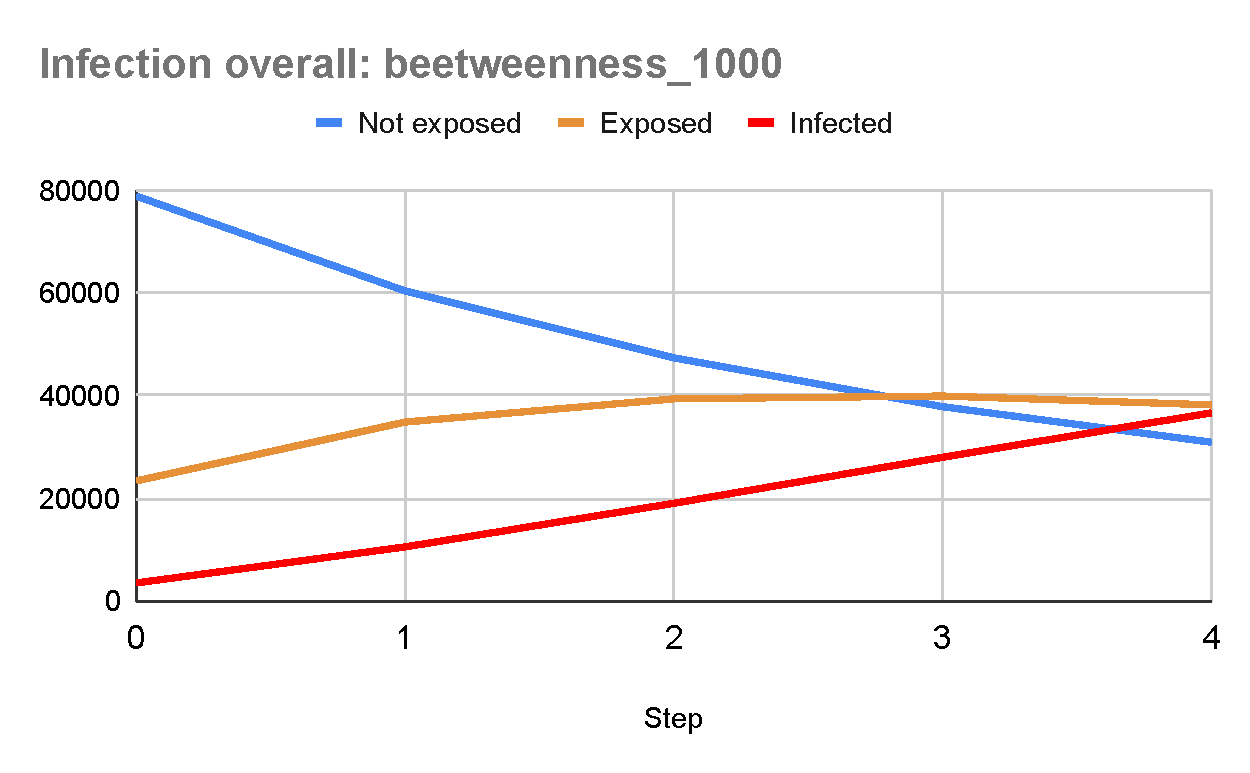
\includegraphics[width=\textwidth]{resources/charts/Infection overall_ beetweenness_1000.pdf}
                \end{minipage}
                \hfill
                \begin{minipage}[c]{0.44\textwidth}
                    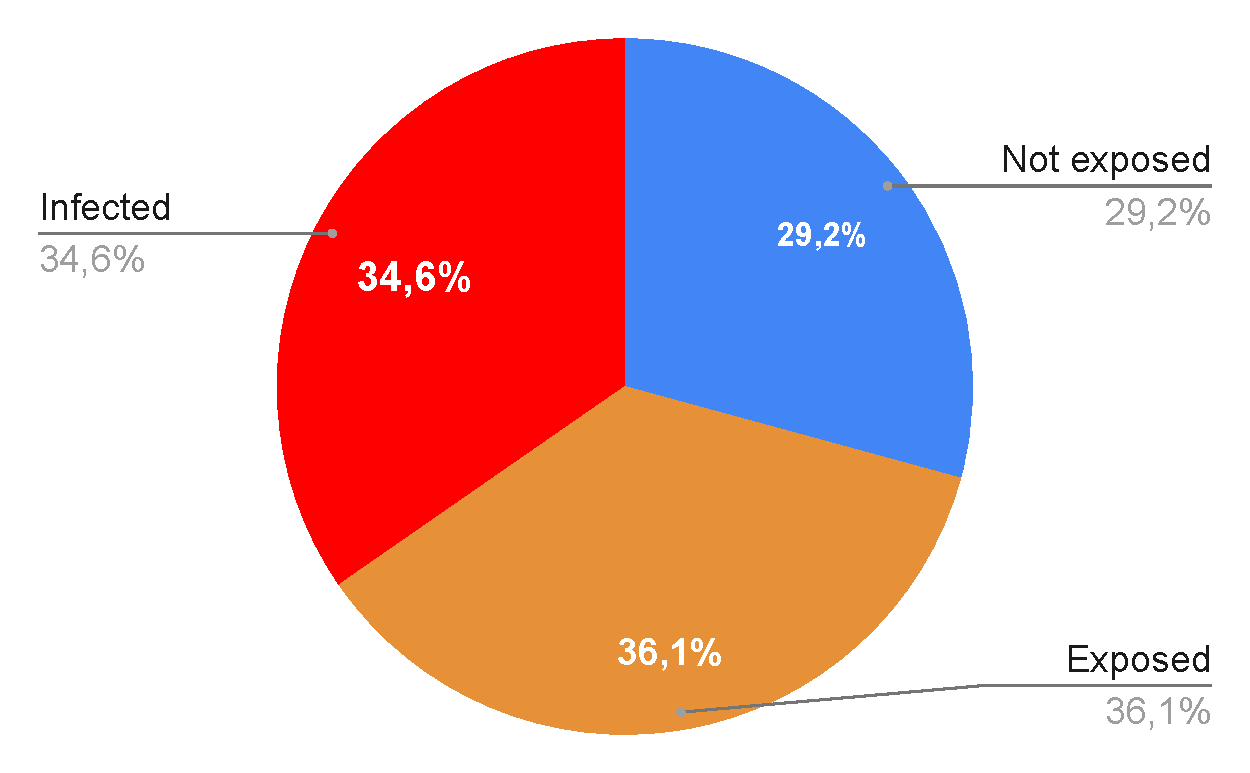
\includegraphics[width=\textwidth]{resources/charts/pie_btw_1000.pdf}
                \end{minipage}
                \caption{Andamento della diffusione dell'informazione. Simulazione betweenness\_100.}
            \end{figure}
            
            
            \begin{table}[H]
                \centering
                \begin{tabular}{l|c|c|c|c|c}
                            & Step 0 & Step 1 & Step 2 & Step 3 & Step 4 \\ \hline
                \textbf{Not exposed} & 78842  & 60377  & 47361  & 37845  & 30926  \\ \hline
                \textbf{Exposed}     & 23402  & 34856  & 39375  & 39927  & 38198  \\ \hline
                \textbf{Infected}    & 3530   & 10541  & 19038  & 28002  & 36650  \\
                \end{tabular}
                \caption{Numero di nodi non esposti/esposti/infetti in relazione agli step della simulazione betweenness\_1000.}
            \end{table}

            \begin{figure}[H]
                \centering
                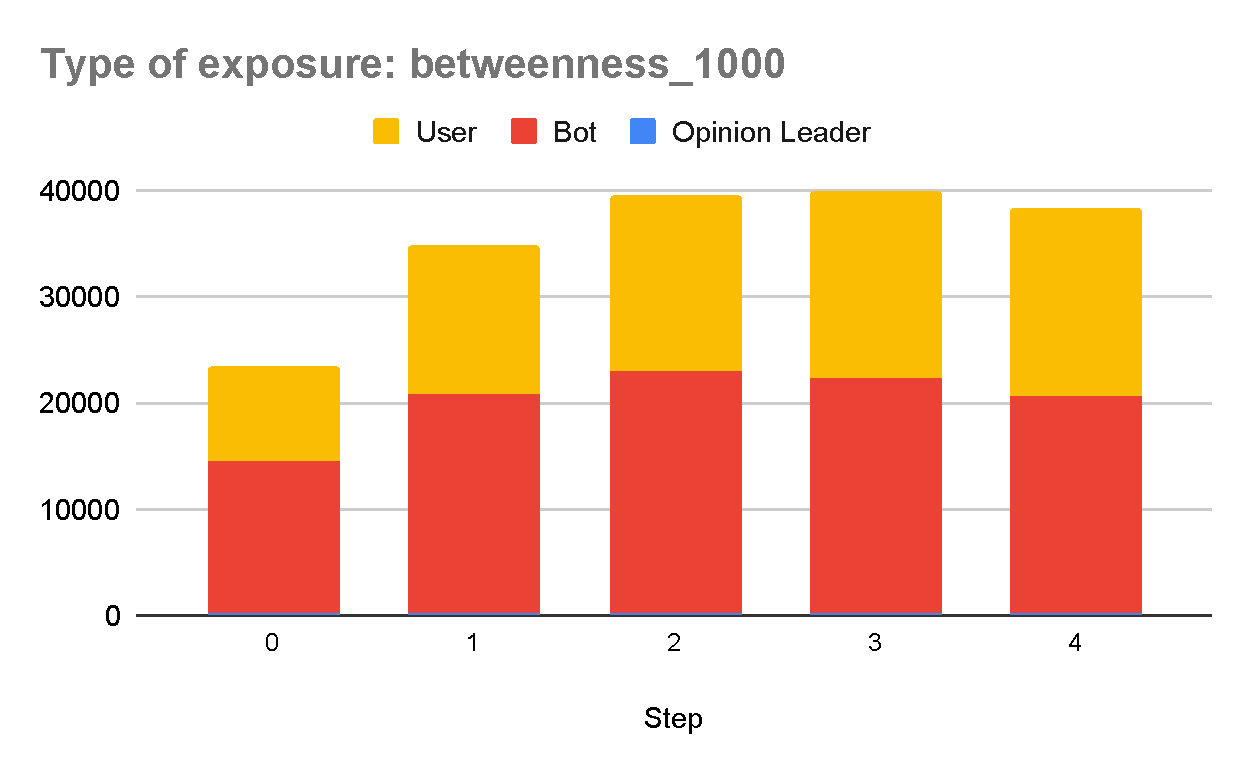
\includegraphics[width=.7\textwidth]{resources/charts/Type of exposure_ betweenness_1000.pdf}
            \caption{Tipologia di esposizione all'informazione durante ogni fase della simulazione betweenness\_1000.}
            \end{figure}
            
            \begin{table}[H]
                \centering
                \begin{tabular}{l|c|c|c|c|c}
                               & Step 0 & Step 1 & Step 2 & Step 3 & Step 4 \\ \hline
                \textbf{Opinion Leader} & 250    & 311    & 326    & 303    & 300    \\ \hline
                \textbf{Bot}            & 14310  & 20642  & 22626  & 22142  & 20370  \\ \hline
                \textbf{User}           & 8842   & 13903  & 16423  & 17482  & 17528  \\
                \end{tabular}
                \caption{Numero di nodi responsabili dell'esposizione in base alla tipologia e allo step di esecuzione della simulazione random\_1000.}
            \end{table}

        \subsubsection{Grafo da 1500 follower}

           \begin{figure}[H]
                \centering
                \begin{minipage}[c]{0.55\textwidth}
                    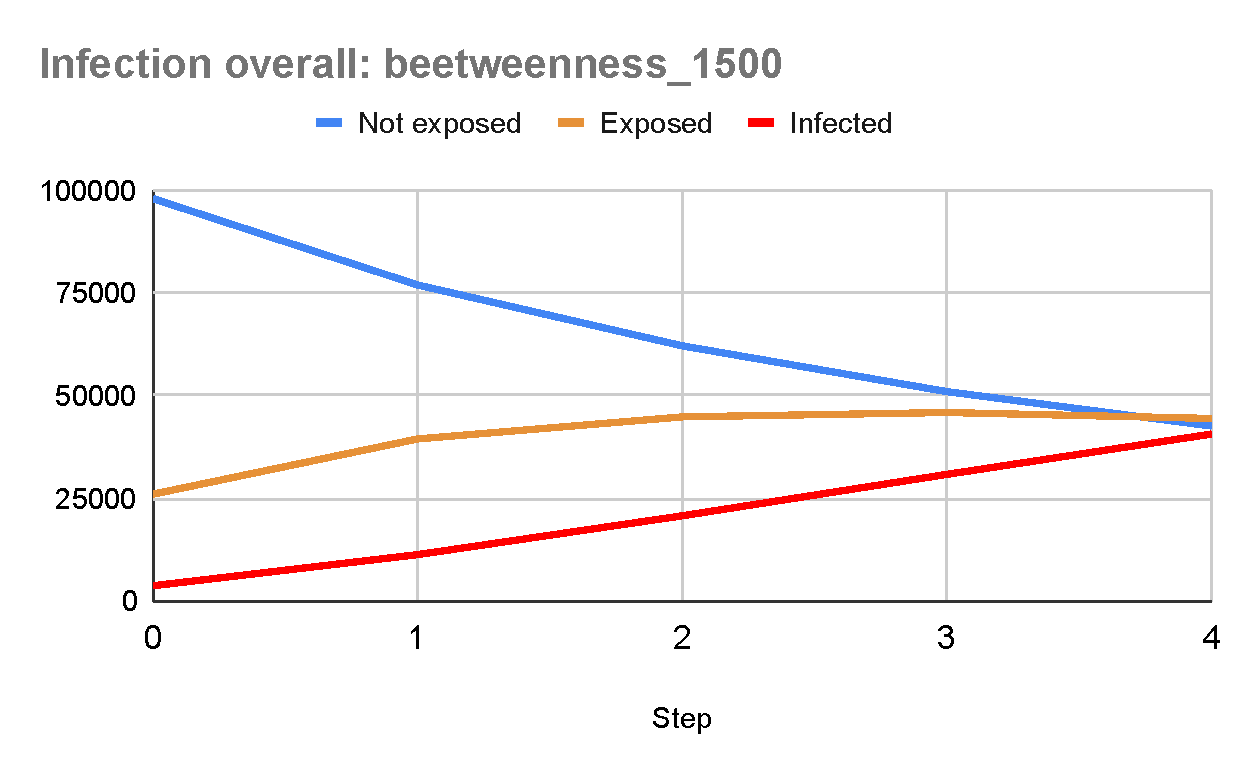
\includegraphics[width=\textwidth]{resources/charts/Infection overall_ beetweenness_1500.pdf}
                \end{minipage}
                \hfill
                \begin{minipage}[c]{0.44\textwidth}
                    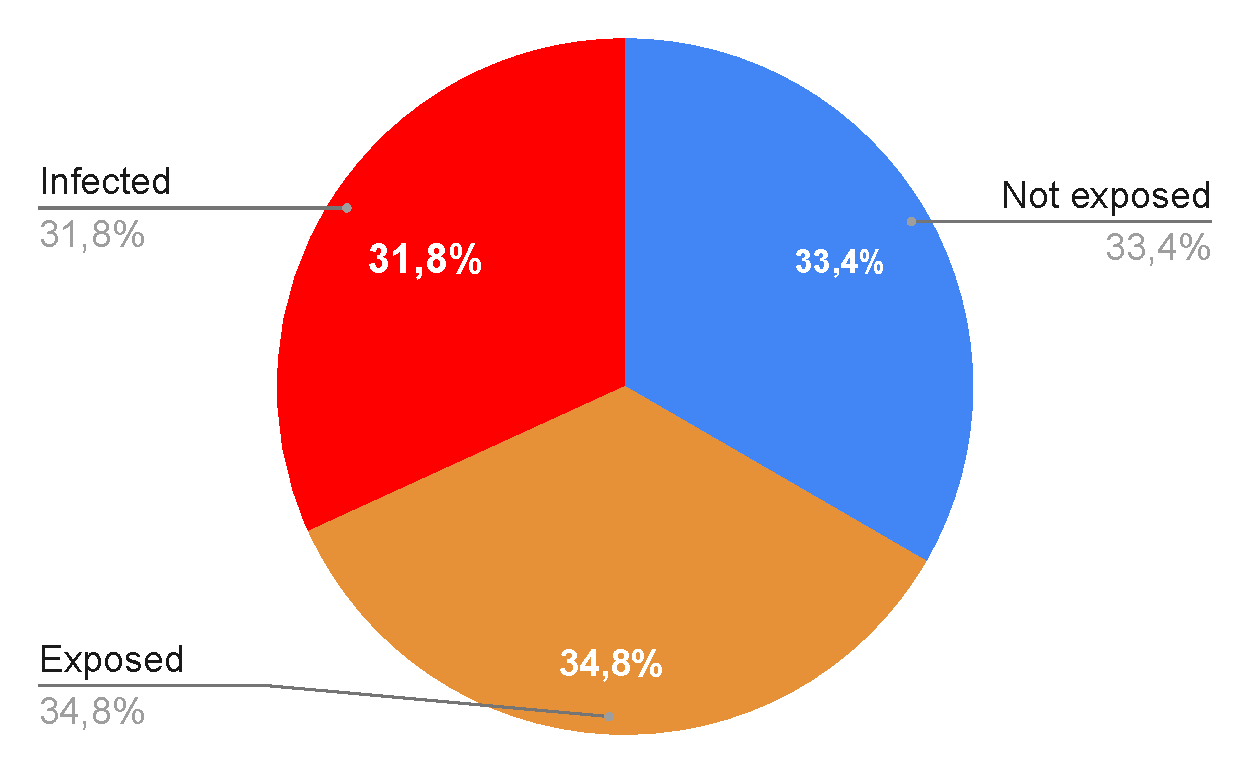
\includegraphics[width=\textwidth]{resources/charts/pie_btw_1500.pdf}
                \end{minipage}
                \caption{Andamento della diffusione dell'informazione. Simulazione betweenness\_1500.}
            \end{figure}
            
            
        \begin{table}[H]
            \centering
            \begin{tabular}{l|c|c|c|c|c}
                        & Step 0 & Step 1 & Step 2 & Step 3 & Step 4 \\ \hline
            \textbf{Not exposed} & 97952  & 76930  & 62122  & 50979  & 42608  \\ \hline
            \textbf{Exposed}     & 26024  & 39468  & 44830  & 45892  & 44446  \\ \hline
            \textbf{Infected}    & 3724   & 11302  & 20748  & 30829  & 40646  \\
            \end{tabular}
            \caption{Tipologia di esposizione all'informazione durante ogni fase della simulazione betweenness\_1500.}
        \end{table}
        
        \begin{figure}[H]
            \centering
            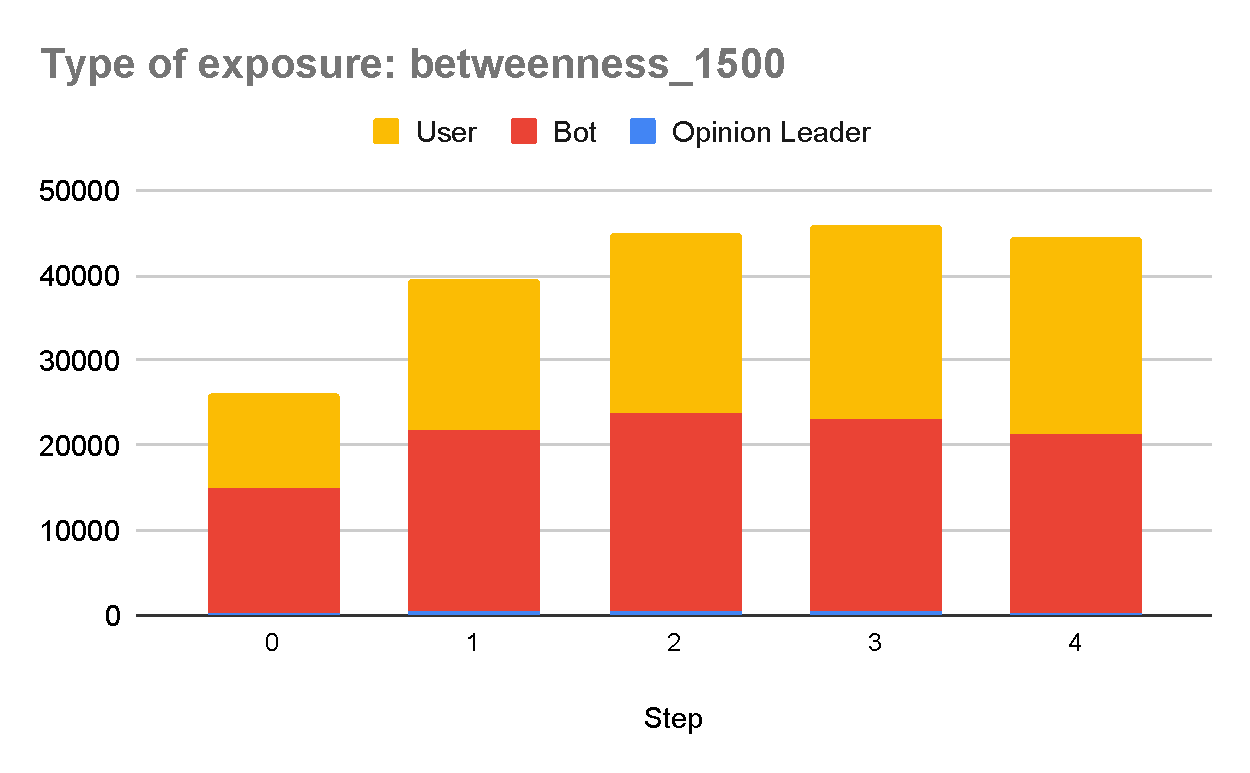
\includegraphics[width=.7\textwidth]{resources/charts/Type of exposure_ betweenness_1500.pdf}
            \caption{Tipologia di esposizione all'informazione durante ogni fase della simulazione betweenness\_1500.}
        \end{figure}
        
        \begin{table}[H]
            \centering
            \begin{tabular}{l|c|c|c|c|c}
                           & Step 0 & Step 1 & Step 2 & Step 3 & Step 4 \\ \hline
            \textbf{Opinion Leader} & 433    & 545    & 545    & 512    & 469    \\ \hline
            \textbf{Bot}            & 14611  & 21355  & 23317  & 22720  & 20955  \\ \hline
            \textbf{User}           & 10980  & 17568  & 20968  & 22660  & 23022  \\
            \end{tabular}
                \caption{Numero di nodi responsabili dell'esposizione in base alla tipologia e allo step di esecuzione della simulazione random\_1500.}
        \end{table}
        
        
        \textbf{Considerazioni simulazioni Betweenness}
        
        I risultati delle simulazioni effettuate considerando la Betweenness come misura di centralità per la scelta della posizione dei Bot dimostrano che questa logica selettiva ha una grande influenza sulla propagazione dell'informazione all'interno della rete. I Bot stessi sono risultati come maggiore causa di esposizione con conseguente innalzamento della percentuale di utenti infetti e esposti rendendo questa quantità significativamente maggiore rispetto a quella degli utenti non esposti. Questi risultati sono osservabili con qualunque dimensione considerata del grafo. 
        
        Infine, si tenga conto che l’eccessiva complessità computazionale richiesta nel calcolo della Betweenness non ci ha permesso di effettuare simulazioni sul grafo dei 2000 follower.
    
        
    \subsection{Eigenvector}
        Vengono di seguito riportati i risultati relativi alle simulazioni basate su scelta del posizionamento dei Bot rispetto alla misura di Eigenvector.
        
        \subsubsection{Grafo da 500 follower}

            \begin{figure}[H]
                \centering
                \begin{minipage}[c]{0.55\textwidth}
                    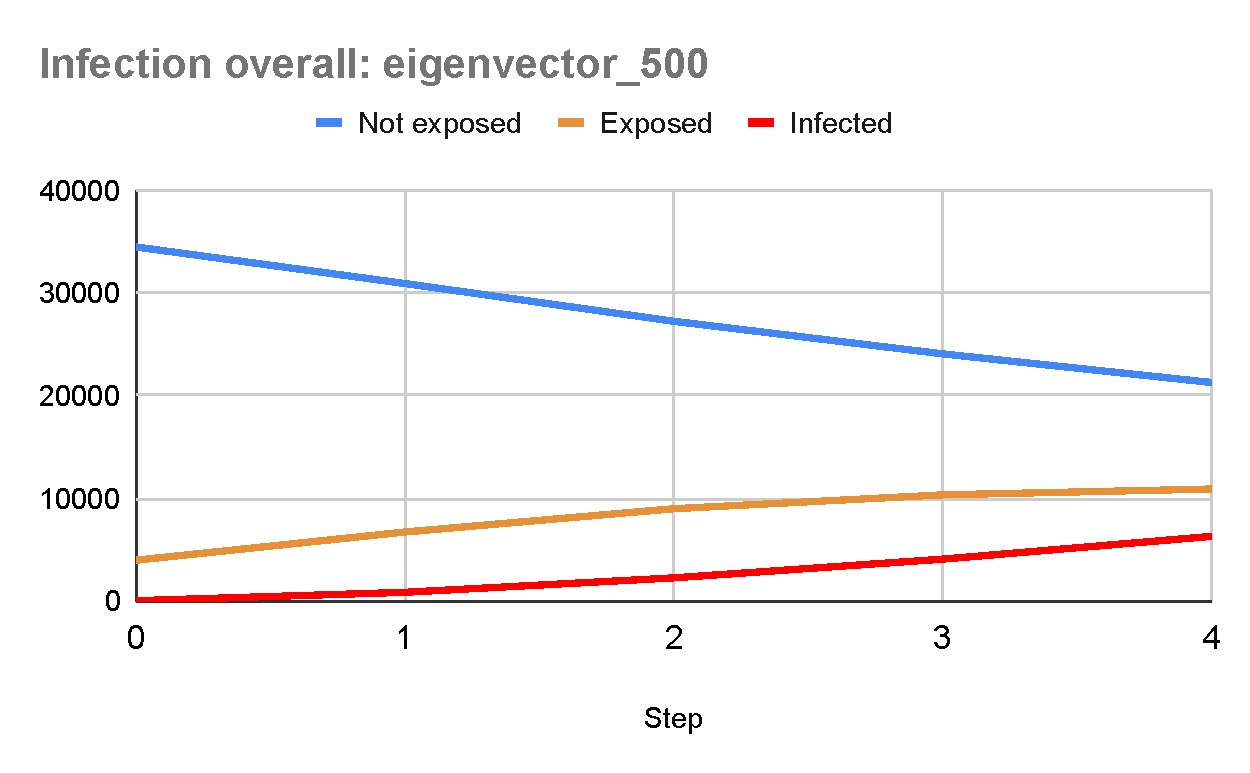
\includegraphics[width=\textwidth]{resources/charts/Infection overall_ eigenvector_500.pdf}
                \end{minipage}
                \hfill
                \begin{minipage}[c]{0.44\textwidth}
                    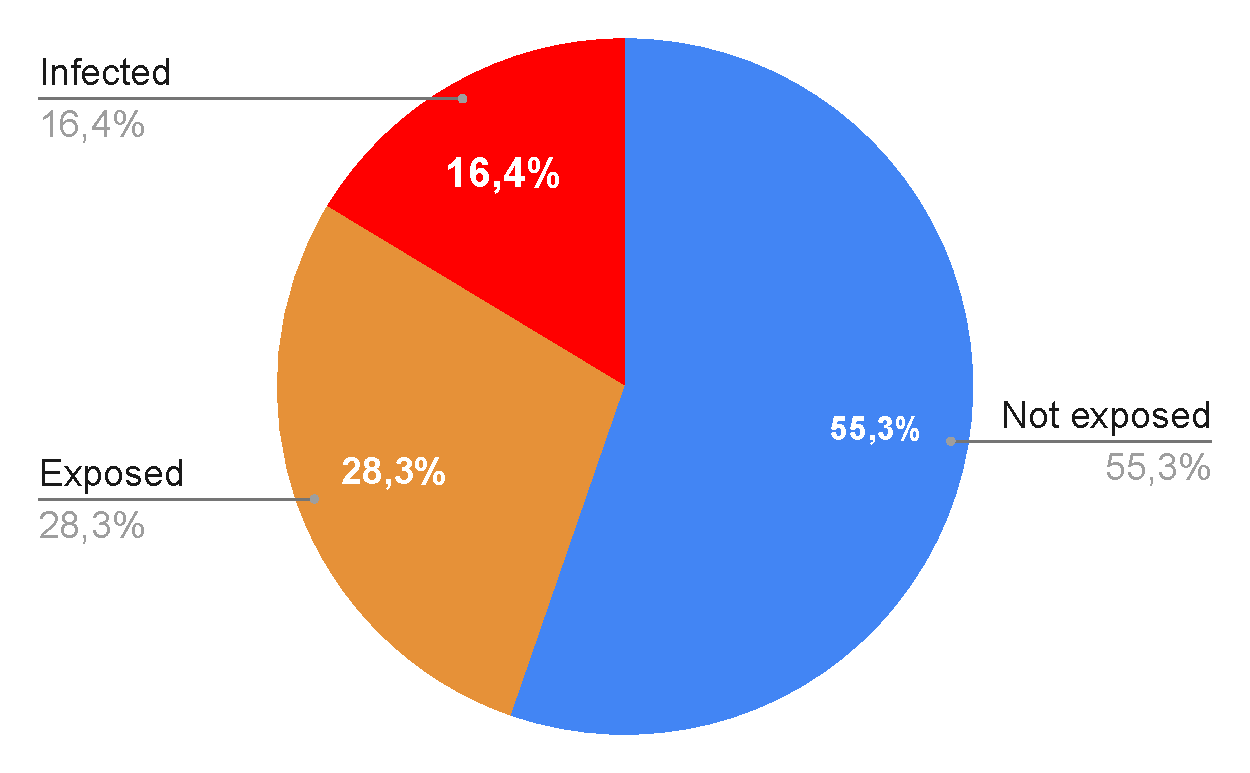
\includegraphics[width=\textwidth]{resources/charts/pie_eig_500.pdf}
                \end{minipage}
                \caption{Andamento della diffusione dell'informazione. Simulazione eigenvector\_500.}
            \end{figure}
            
        \begin{table}[H]
            \centering
            \begin{tabular}{l|c|c|c|c|c}
                        & Step 0 & Step 1 & Step 2 & Step 3 & Step 4 \\ \hline
            \textbf{Not exposed} & 34472  & 30910  & 27239  & 24068  & 21281  \\ \hline
            \textbf{Exposed}     & 3980   & 6724   & 8989   & 10338  & 10908  \\ \hline
            \textbf{Infected}    & 33     & 851    & 2257   & 4079   & 6296   \\
            \end{tabular}
            \caption{Tipologia di esposizione all'informazione durante ogni fase della simulazione eigenvector\_500.}
        \end{table}
        
        \begin{figure}[H]
            \centering
            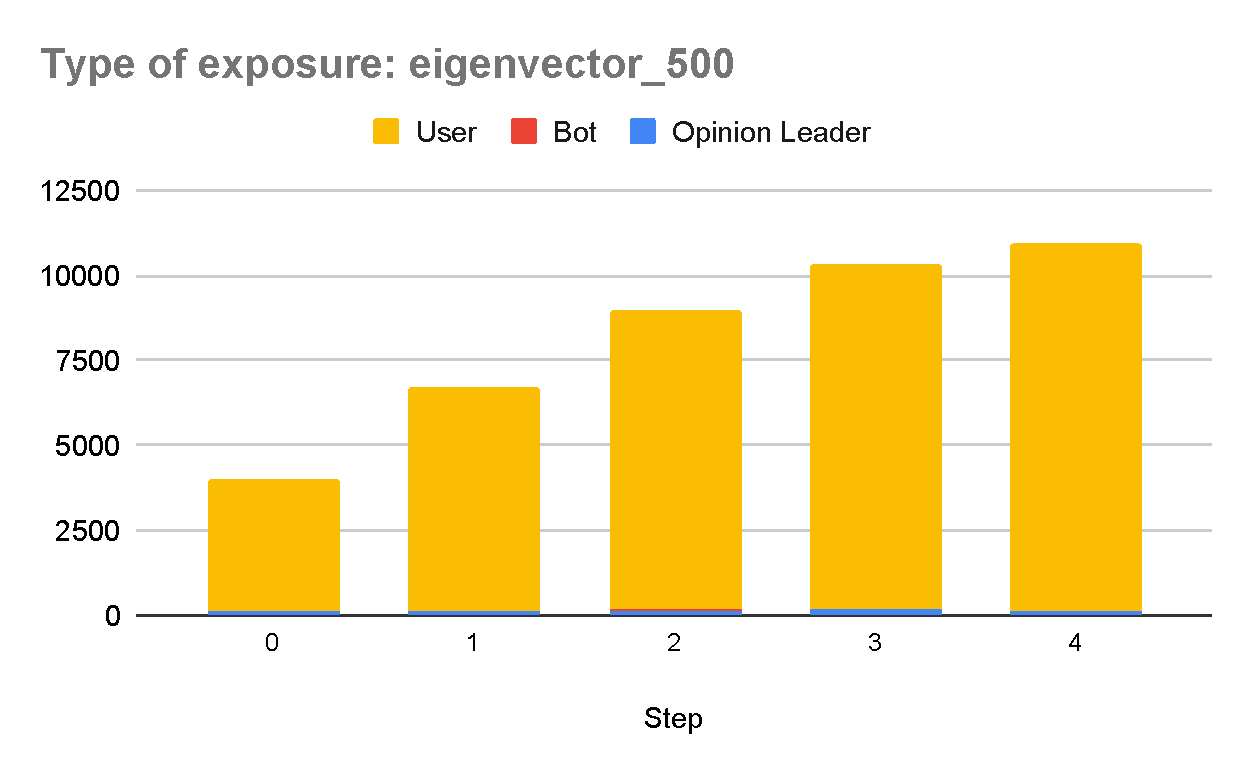
\includegraphics[width=.7\textwidth]{resources/charts/Type of exposure_ eigenvector_500.pdf}
            \caption{Tipologia di esposizione all'informazione durante ogni fase della simulazione eigenvector\_500.}
        \end{figure}
        
        \begin{table}[H]
            \centering
            \begin{tabular}{l|c|c|c|c|c}
                           & Step 0 & Step 1 & Step 2 & Step 3 & Step 4 \\ \hline
            \textbf{Opinion Leader} & 123    & 165    & 179    & 183    & 165    \\ \hline
            \textbf{Bot}            & 10     & 10     & 9      & 8      & 8      \\ \hline
            \textbf{User}           & 3847   & 6549   & 8801   & 10147  & 10735  \\
            \end{tabular}
            \caption{Numero di nodi responsabili dell'esposizione in base alla tipologia e allo step di esecuzione della simulazione eigenvector\_500.}
        \end{table}

        \subsubsection{Grafo da 1000 follower}

            \begin{figure}[H]
                \centering
                \begin{minipage}[c]{0.55\textwidth}
                    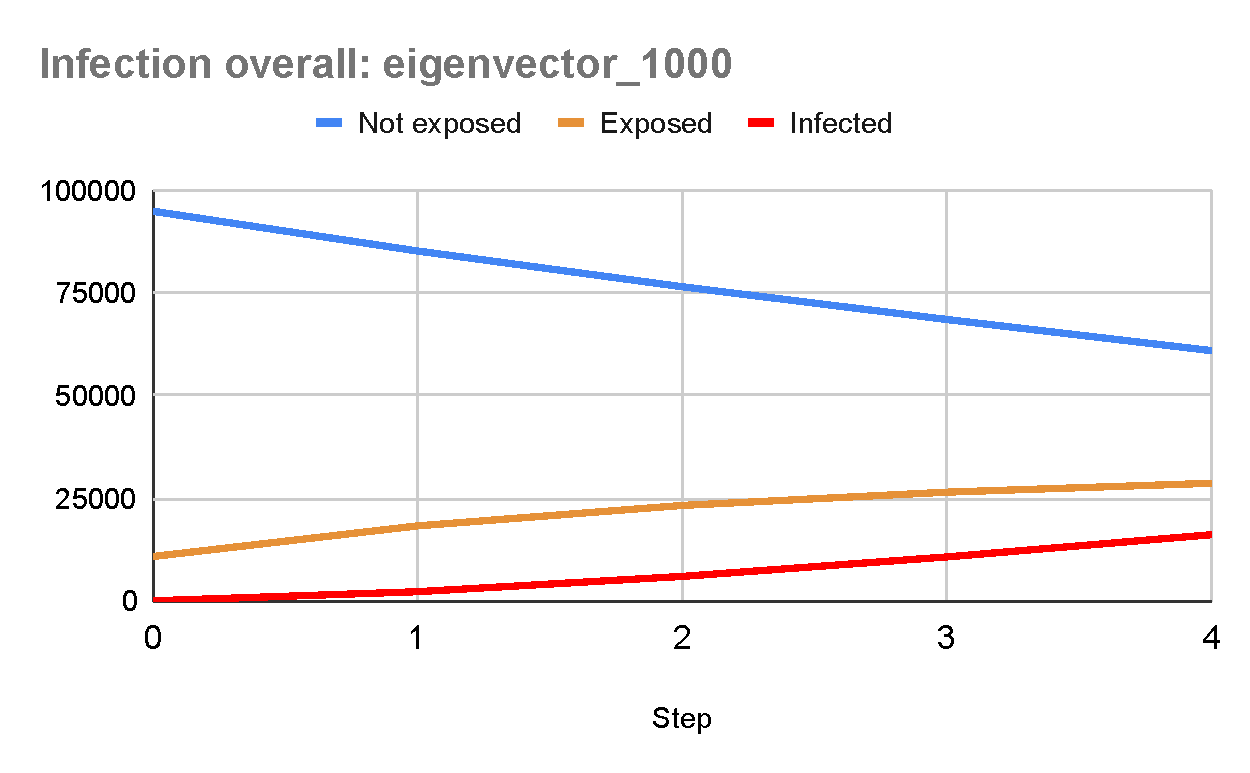
\includegraphics[width=\textwidth]{resources/charts/Infection overall_ eigenvector_1000.pdf}
                \end{minipage}
                \hfill
                \begin{minipage}[c]{0.44\textwidth}
                    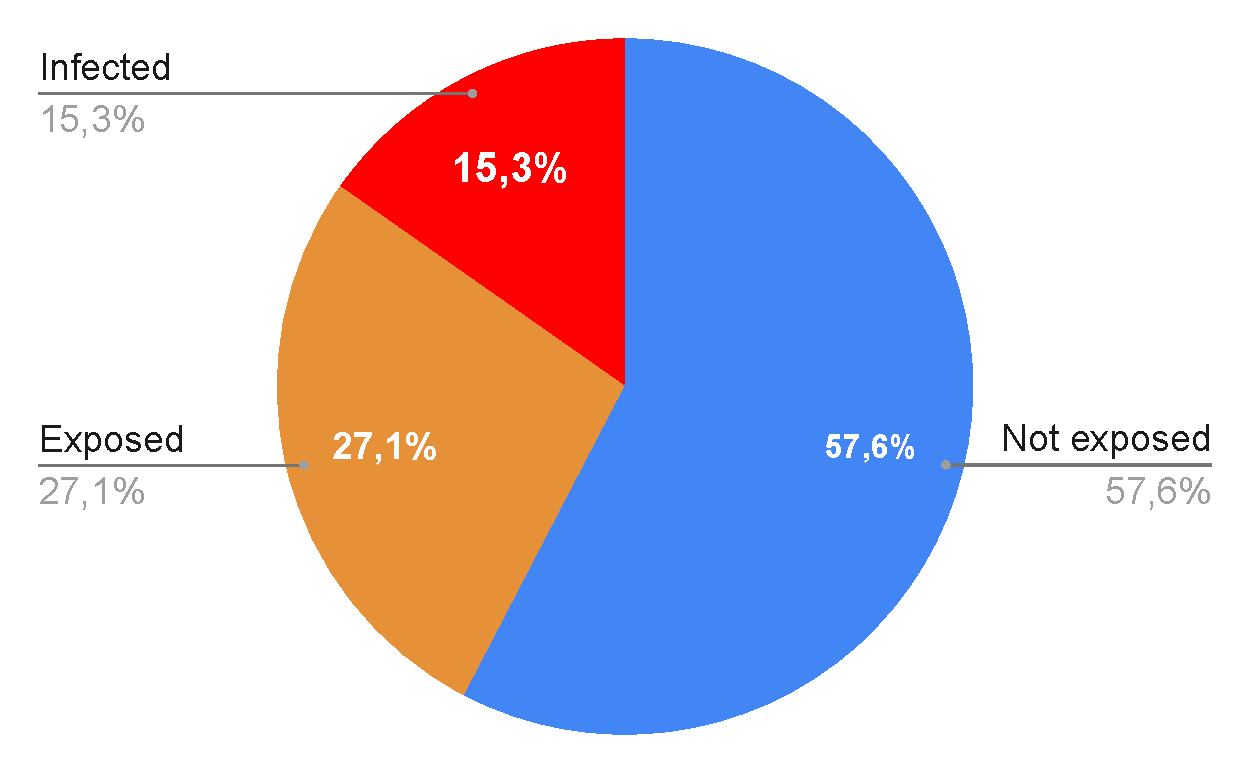
\includegraphics[width=\textwidth]{resources/charts/pie_eig_1000.pdf}
                \end{minipage}
                \caption{Andamento della diffusione dell'informazione. Simulazione eigenvector\_1000.}
            \end{figure}
            
        \begin{table}[H]
            \centering
            \begin{tabular}{l|c|c|c|c|c}
                        & Step 0 & Step 1 & Step 2 & Step 3 & Step 4 \\ \hline
            \textbf{Not exposed} & 94882  & 85205  & 76507  & 68538  & 60957  \\ \hline
            \textbf{Exposed}     & 10841  & 18297  & 23274  & 26501  & 28671  \\ \hline
            \textbf{Infected}    & 51     & 2272   & 5993   & 10735  & 16146  \\
            \end{tabular}
            \caption{Numero di nodi non esposti/esposti/infetti in relazione agli step della simulazione eigenvector\_1000.}
        \end{table}
        
        \begin{figure}[H]
            \centering
            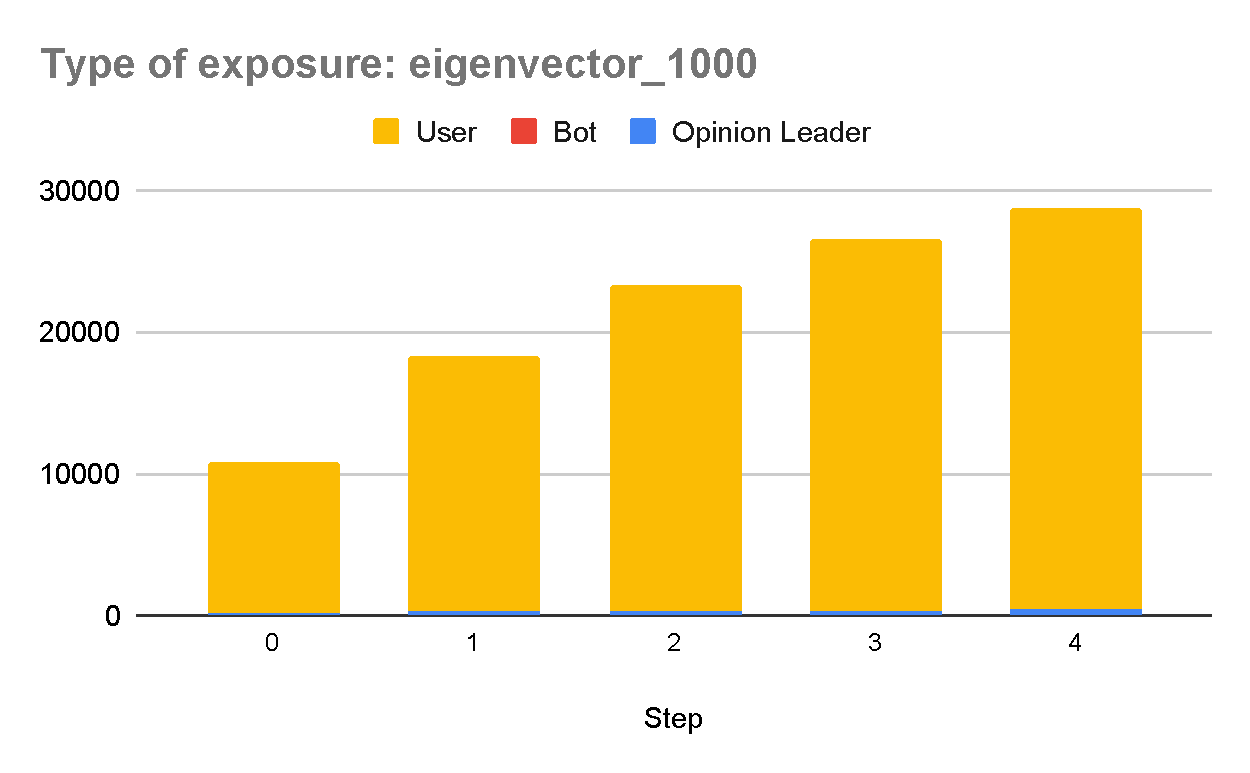
\includegraphics[width=.7\textwidth]{resources/charts/Type of exposure_ eigenvector_1000.pdf}
            \caption{Tipologia di esposizione all'informazione durante ogni fase della simulazione eigenvector\_1000.}
        \end{figure}
        
        \begin{table}[H]
            \centering
            \begin{tabular}{l|c|c|c|c|c}
                           & Step 0 & Step 1 & Step 2 & Step 3 & Step 4 \\ \hline
            \textbf{Opinion Leader} & 259    & 321    & 346    & 363    & 473    \\ \hline
            \textbf{Bot}            & 2      & 5      & 4      & 4      & 7      \\ \hline
            \textbf{User}           & 10580  & 17971  & 22924  & 26134  & 28191  \\
            \end{tabular}
            \caption{Numero di nodi responsabili dell'esposizione in base alla tipologia e allo step di esecuzione della simulazione eigenvector\_1000.}
        \end{table}

        \subsubsection{Grafo da 1500 follower}

            \begin{figure}[H]
                \centering
                \begin{minipage}[c]{0.55\textwidth}
                    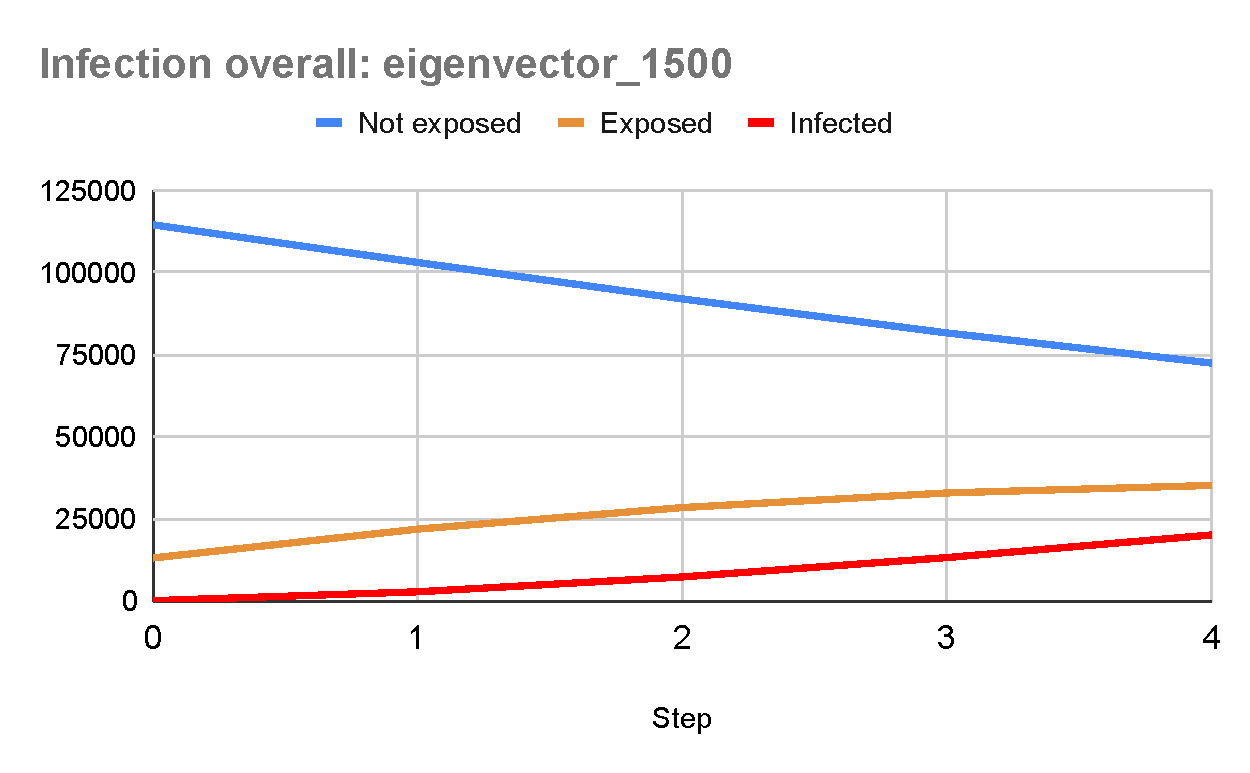
\includegraphics[width=\textwidth]{resources/charts/Infection overall_ eigenvector_1500.pdf}
                \end{minipage}
                \hfill
                \begin{minipage}[c]{0.44\textwidth}
                    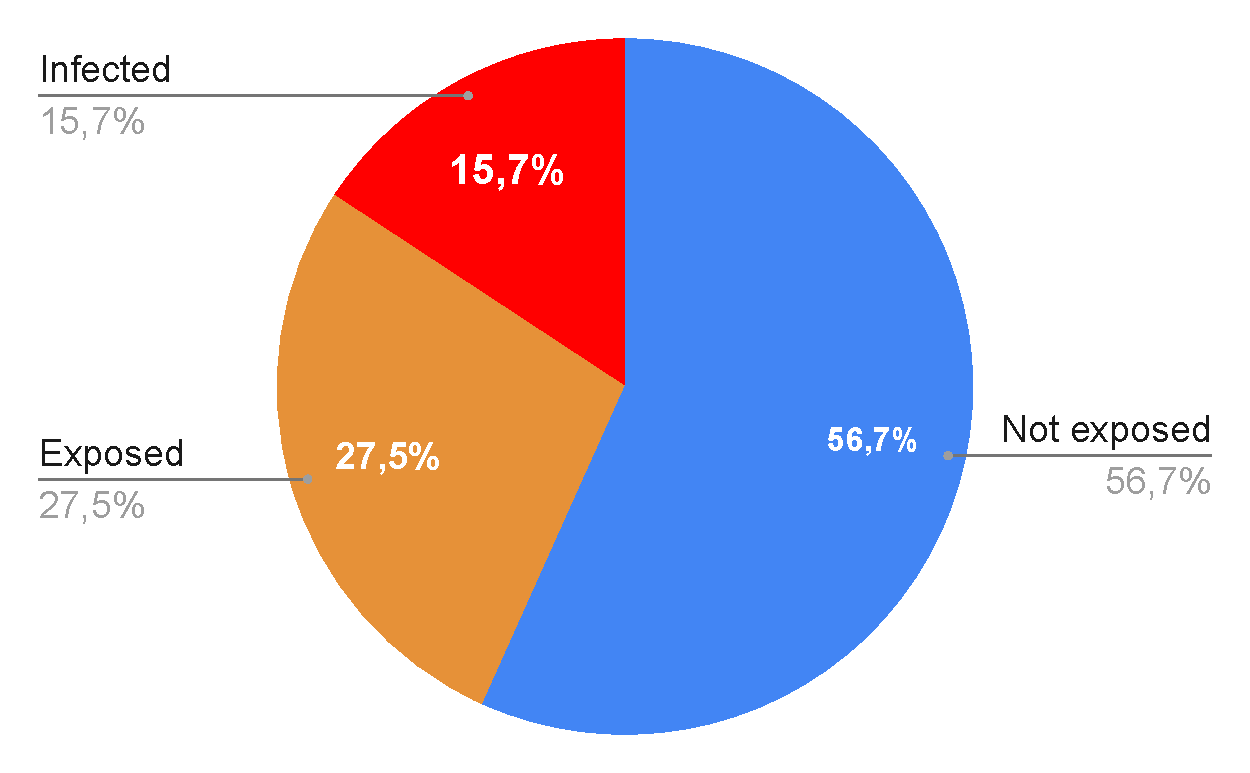
\includegraphics[width=\textwidth]{resources/charts/pie_eig_1500.pdf}
                \end{minipage}
                \caption{Andamento della diffusione dell'informazione. Simulazione eigenvector\_1500.}
            \end{figure}
        
        \begin{table}[H]
            \centering
            \begin{tabular}{l|c|c|c|c|c}
                        & Step 0 & Step 1 & Step 2 & Step 3 & Step 4 \\ \hline
            \textbf{Not exposed} & 114474 & 103011 & 91937  & 81591  & 72417  \\ \hline
            \textbf{Exposed}     & 13113  & 21881  & 28436  & 32890  & 35178  \\ \hline
            \textbf{Infected}    & 113    & 2808   & 7327   & 13219  & 20105  \\
            \end{tabular}
            \caption{Tipologia di esposizione all'informazione durante ogni fase della simulazione eigenvector\_1500.}
        \end{table}
        
        \begin{figure}[H]
            \centering
            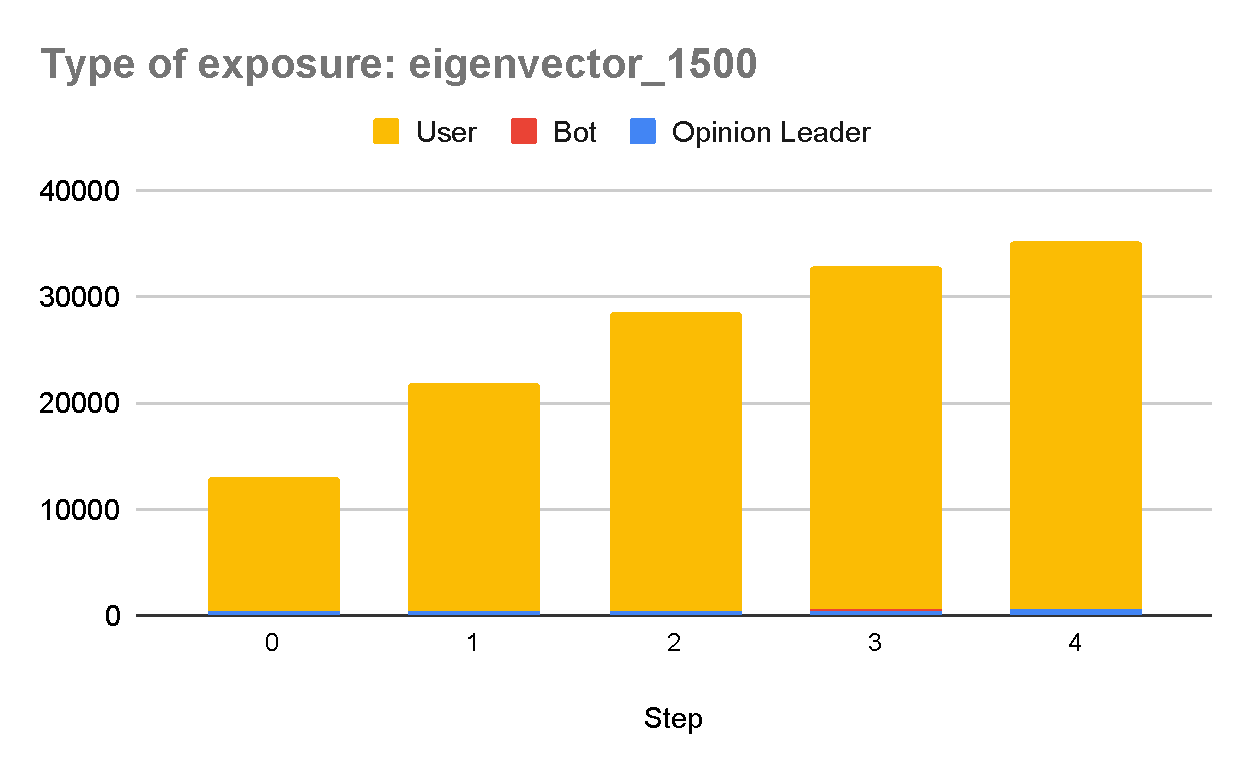
\includegraphics[width=.7\textwidth]{resources/charts/Type of exposure_ eigenvector_1500.pdf}
            \caption{Tipologia di esposizione all'informazione durante ogni fase della simulazione eigenvector\_1500.}
        \end{figure}
        
        \begin{table}[H]
            \centering
            \begin{tabular}{l|c|c|c|c|c}
                           & Step 0 & Step 1 & Step 2 & Step 3 & Step 4 \\ \hline
            \textbf{Opinion Leader} & 415    & 526    & 542    & 571    & 592    \\ \hline
            \textbf{Bot}            & 4      & 3      & 7      & 8      & 7      \\ \hline
            \textbf{User}           & 12694  & 21352  & 27887  & 32311  & 34579  \\
            \end{tabular}
            \caption{Numero di nodi responsabili dell'esposizione in base alla tipologia e allo step di esecuzione della simulazione eigenvector\_1500.}
        \end{table}

        \subsubsection{Grafo da 2000 follower}

            \begin{figure}[H]
                \centering
                \begin{minipage}[c]{0.55\textwidth}
                    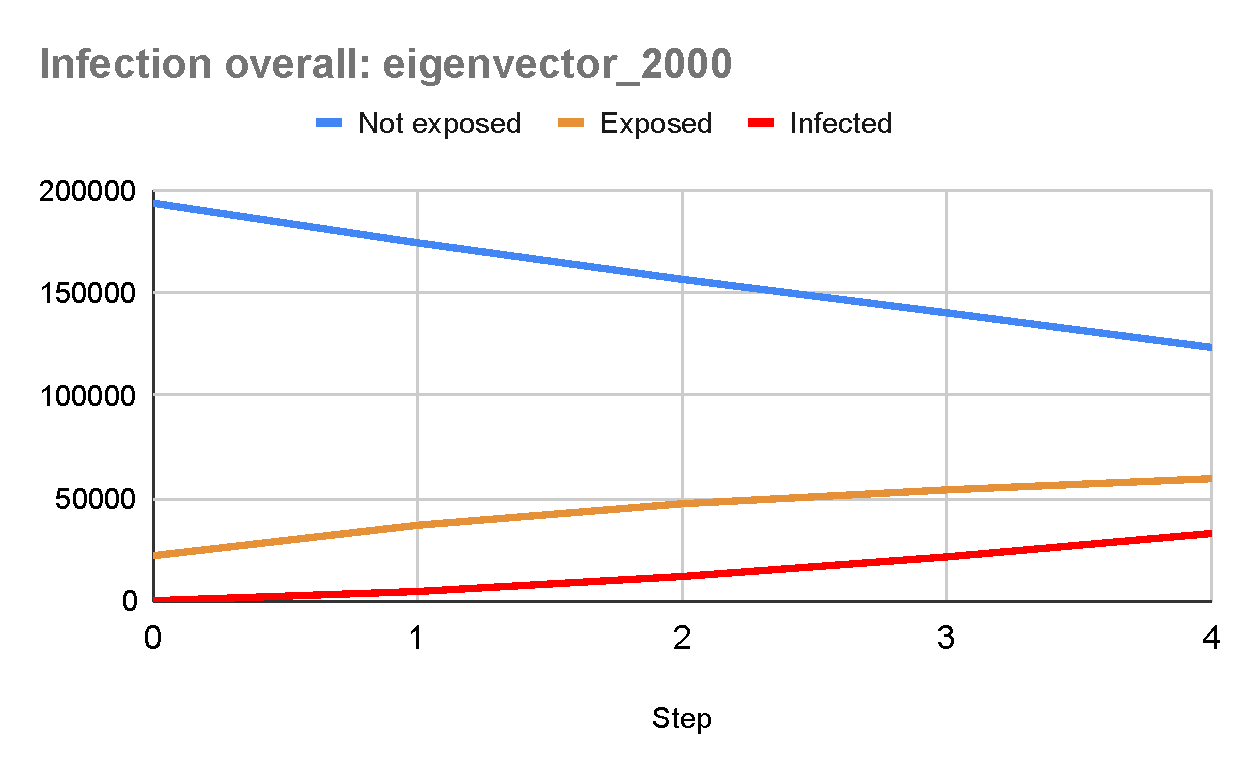
\includegraphics[width=\textwidth]{resources/charts/Infection overall_ eigenvector_2000.pdf}
                \end{minipage}
                \hfill
                \begin{minipage}[c]{0.44\textwidth}
                    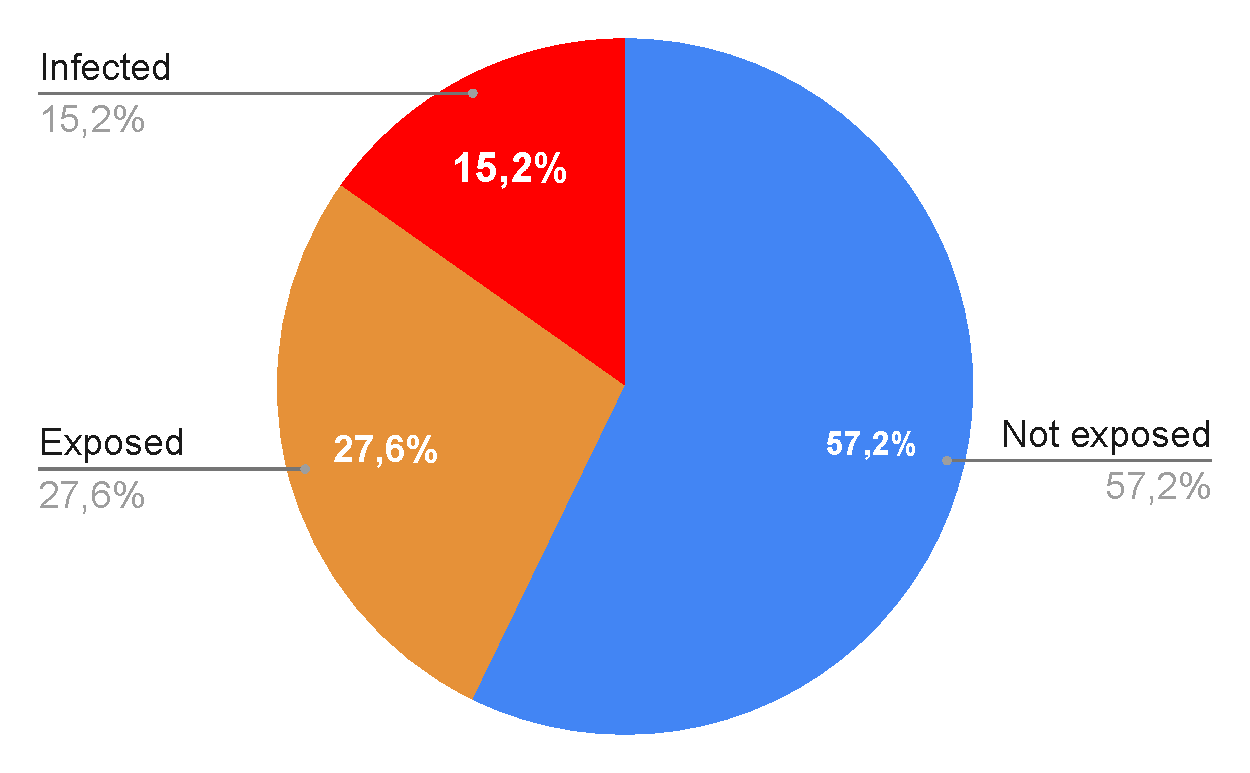
\includegraphics[width=\textwidth]{resources/charts/pie_eig_2000.pdf}
                \end{minipage}
                \caption{Andamento della diffusione dell'informazione. Simulazione eigenvector\_2000.}
            \end{figure}
        
        \begin{table}[H]
            \centering
            \begin{tabular}{l|c|c|c|c|c}
                        & Step 0 & Step 1 & Step 2 & Step 3 & Step 4 \\ \hline
            \textbf{Not exposed} & 193700 & 174382 & 156612 & 140306 & 123490 \\ \hline
            \textbf{Exposed}     & 22060  & 36892  & 47361  & 54124  & 59550  \\ \hline
            \textbf{Infected}    & 150    & 4636   & 11937  & 21480  & 32870  \\
            \end{tabular}
            \caption{Tipologia di esposizione all'informazione durante ogni fase della simulazione eigenvector\_2000.}
        \end{table}
        
        \begin{figure}[H]
            \centering
            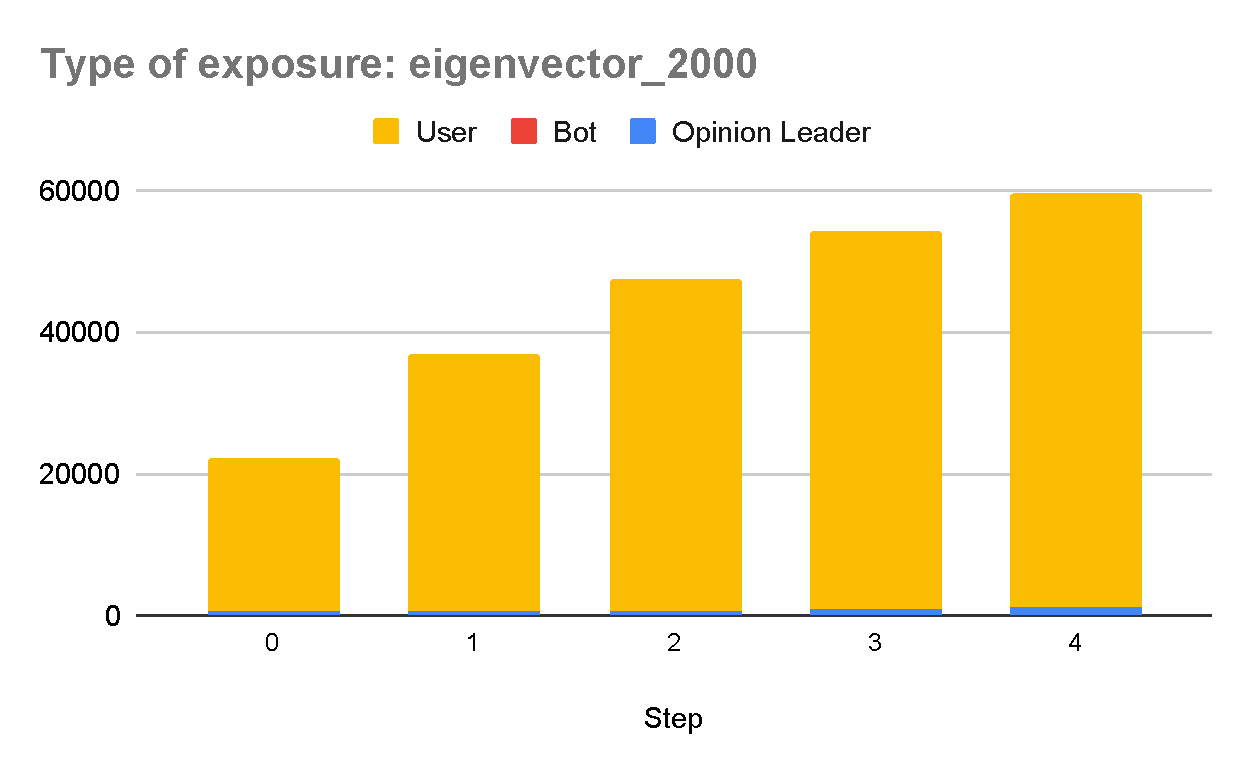
\includegraphics[width=.7\textwidth]{resources/charts/Type of exposure_ eigenvector_2000.pdf}
            \caption{Tipologia di esposizione all'informazione durante ogni fase della simulazione eigenvector\_2000.}
        \end{figure}
        
        \begin{table}[H]
            \centering
            \begin{tabular}{l|c|c|c|c|c}
                           & Step 0 & Step 1 & Step 2 & Step 3 & Step 4 \\ \hline
            \textbf{Opinion Leader} & 618    & 736    & 792    & 898    & 1308   \\ \hline
            \textbf{Bot}            & 0      & 1      & 1      & 1      & 1      \\ \hline
            \textbf{User}           & 21442  & 36155  & 46568  & 53225  & 58241  \\
            \end{tabular}
            \caption{Numero di nodi responsabili dell'esposizione in base alla tipologia e allo step di esecuzione della simulazione eigenvector\_2000.}
        \end{table}

        \textbf{Considerazioni simulazioni Eigenvector}
        
        Selezionando i Bot secondo la centralità basata su autovettori si hanno risultati inaspettatamente simili a quelli ottenuti selezionando i Bot in maniera randomica, contribuendo in modo minimo alla diffusione della news all'interno del grafo. Come nelle simulazioni precedenti riferite alla selezione randomica, la percentuale di utenti non esposti è risultata superiore a  quella degli utenti esposti o infetti.
        
        Concludiamo affermando che anche in questo caso la differente topologia del grafo non ha influenzato i risultati delle simulazioni.